\documentclass[aspectratio=169, 12pt]{beamer}

\usepackage{lmodern}
\usepackage{hyperref}
\usepackage{graphicx}
\usepackage{booktabs}
\usepackage[authordate,maxcitenames=1,backend=biber,doi=false,isbn=false,url=false]{biblatex-chicago}
\renewcommand*{\nameyeardelim}{\addcomma\addspace}
% \addbibresource{discrimination.bib}

\usepackage{amsmath}
\usepackage{amssymb}
\usepackage{amsthm}
\usepackage{bm}
\usepackage{bbm}
\usepackage{mathtools}
\setbeamertemplate{theorems}[numbered]
\newtheorem{proposition}{Proposition}
\newtheorem{assumption}{Assumption}

\DeclareMathOperator*{\plim}{plim}
\DeclareMathOperator*{\var}{var}
\DeclareMathOperator*{\cov}{cov}

\newcommand{\indep}{\perp \!\!\! \perp}
\newcommand{\R}{\mathbb{R}}
\newcommand{\I}{\mathbbm{1}}
\newcommand{\argmax}{\mathop{\rm arg~max}\limits}
\newcommand{\argmin}{\mathop{\rm arg~min}\limits}

% preambles for tables
\usepackage{booktabs}
\usepackage{adjustbox}
\usepackage{caption}
\captionsetup{labelformat=empty}
\usepackage{tikz}
\usetikzlibrary{calc}
\newcommand{\tikzmark}[1]{\tikz[overlay,remember picture] \node (#1) {};}
\newcommand{\DrawBox}[1][]{%
    \tikz[overlay,remember picture]{
    \draw[#1,thick]
      ($(left)+(-0.2em,0.9em)$) rectangle
      ($(right)+(0.2em,-0.3em)$);}
}
\usepackage[group-separator={,}]{siunitx}
\usepackage{longtable}
\usepackage{rotating}
\usepackage{threeparttable}

\newcommand{\backupbegin}{
   \newcounter{framenumberappendix}
   \setcounter{framenumberappendix}{\value{framenumber}}
}
\newcommand{\backupend}{
   \addtocounter{framenumberappendix}{-\value{framenumber}}
   \addtocounter{framenumber}{\value{framenumberappendix}} 
}

\usepackage{silence}
\WarningFilter{latexfont}{Font shape}
\WarningFilter{biblatex}{Patching footnotes failed}

\usetheme{Boadilla}
\usecolortheme{orchid}
\usefonttheme{professionalfonts}

\setbeamertemplate{section in toc}[sections numbered]
\setbeamertemplate{itemize item}[default]
\setbeamertemplate{itemize subitem}[square]
\setbeamertemplate{enumerate items}[default]
\setbeamertemplate{navigation symbols}{}
\setbeamertemplate{itemize/enumerate body begin}{\normalsize}
\setbeamertemplate{itemize/enumerate subbody begin}{\normalsize}
\setbeamertemplate{itemize/enumerate subsubbody begin}{\normalsize}
\setbeamerfont{title}{size=\large}
\setbeamerfont{institute}{size=\small}
\setbeamercovered{dynamic}

\title[Topics on R]{Topics on R}
\author[Konan Hara]{Konan Hara}
\institute[Arizona]{University of Arizona}
\date{September 8, 2021}
\begin{document}

	\begin{frame}[plain]
	\titlepage
	\end{frame}

	\begin{frame}
	\frametitle{Why Use R?---Popularity in Data Science}
	\begin{figure}
	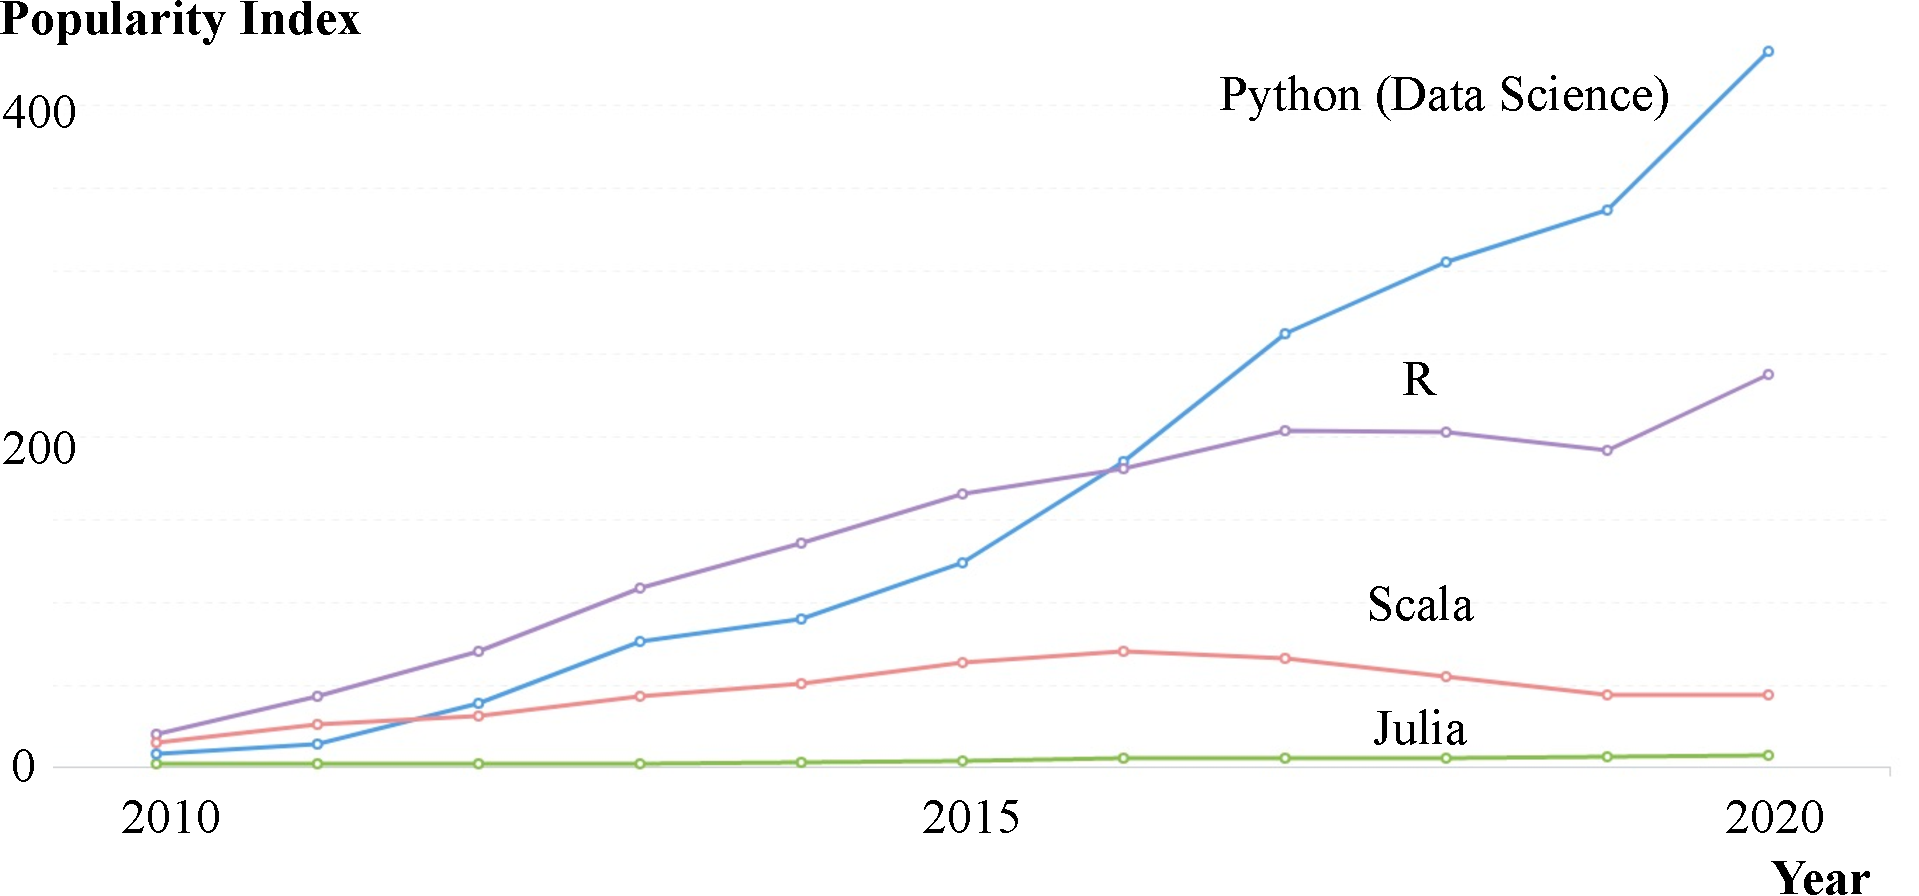
\includegraphics[width=0.8\textwidth]{fig/Popularity_Ranking_Programming_Languages_Data_Science-crop.pdf}
	\end{figure}
	\vspace*{-10pt}
	\begin{itemize}
	\item Popularity index is calculated based on \# questions asked daily, \# daily distinct users, and \# view counts of questions in Stack Overflow. [\href{https://towardsdatascience.com/popularity-ranking-of-programming-languages-72bcf697ea20}{\underline{Ref}}]
	\item Proprietary languages like Stata, Matlab, and SAS do not appear here.
	\end{itemize}

	\end{frame}

	\begin{frame}
	\frametitle{Why Use R?---R vs. Python}
	\begin{itemize}
	\item General idea:
	\begin{itemize}
	\item R's functionality was developed with statisticians in mind
	\item Python is often praised for being a general-purpose language with an easy-to-understand syntax
	\end{itemize}
	\item Factors that may affect your decision:
	\begin{enumerate}
	\item Which language do your colleagues use?
	\item What problems do you want to solve and what tasks do you need to accomplish?
	\item What are the net costs of learning a language?
	\item What are the commonly used tool(s) in your field?
	\end{enumerate}
	\end{itemize}

	\end{frame}

	\begin{frame}
	\frametitle{Why Use R?---R vs. Python}
	\begin{itemize}
	\item R advantages:
	\begin{itemize}
	\item R is easier to learn if you have no coding experience.
	\item Widely considered the best tool for making beautiful graphs and visualizations.
	\item Has many functionalities for data/statistical analysis
	\item Statistical models can be written with only a few lines.
	\end{itemize}
	\item Python advantages:
	\begin{itemize}
	\item General-purpose programming languages are useful beyond just data analysis.
	\item Python’s focus on readability and simplicity means its learning curve is relatively linear and smooth.
	\item Great for mathematical computation and learning how algorithms work.
	\end{itemize}
	\end{itemize}

	\end{frame}

	\begin{frame}
	\frametitle{Why Use R?---R vs. Python}
	\begin{itemize}
	\item R disadvantages:
	\begin{itemize}
	\item Finding the right packages to use in R may be time consuming.
	\item R can be considered slow if code is written poorly.
	\item Not as popular as Python for deep learning and NLP.
	\end{itemize}
	\item Python disadvantages:
	\begin{itemize}
	\item Python doesn’t have as many libraries for data science as R.
	\item Visualizations are more convoluted in Python than in R, and results are not as eye-pleasing or informative.
	\end{itemize}
	\end{itemize}

	\end{frame}

	\begin{frame}
	\frametitle{Good Programming Habits}
	A good code is:
	\begin{itemize}
	\item Easy to maintain
	\item Easy to extend
	\item Easy to understand...even after a six month break!
	\item Straight-forward and direct...no side-effects or surprises!
	\item Reads like English (or some other human language)
	\end{itemize}

	\end{frame}

	\begin{frame}
	\frametitle{Good Programming Habits}
	\begin{itemize}
	\item Naming of functions, variables, and filenames: e.g., 
	\begin{itemize}
	\item Begin or end function names with a verb.
	\item Separate each word by CamelCase, `\_', or `.'.
	\item Examples, CalcValueFunc; calc\_value\_func.
	\end{itemize}
	\item Comments: 
	\begin{itemize}
	\item Write why you did something rather than what you did.
	\item One variable definition per line.
	\end{itemize} 
	\item Respect the local coding convention when working on code.
	\begin{itemize}
	\item E.g., \href{https://google.github.io/styleguide/Rguide.html}{\underline{Google’s R Style Guide}}
	\end{itemize}
	\item Advanced habits:
	\begin{itemize}
	\item Code publication
	\item README file
	\item Modification history
	\item Reproducible research

	\end{itemize}
	\end{itemize}

	\end{frame}

	\begin{frame}
	\begin{figure}
	
\includegraphics[width=0.8\textwidth]{fig/Sanchez_title.png}
	\end{figure}

	\end{frame}

	\begin{frame}
	\frametitle{GitHub Can Help You: Code Publication}
	\begin{figure}
	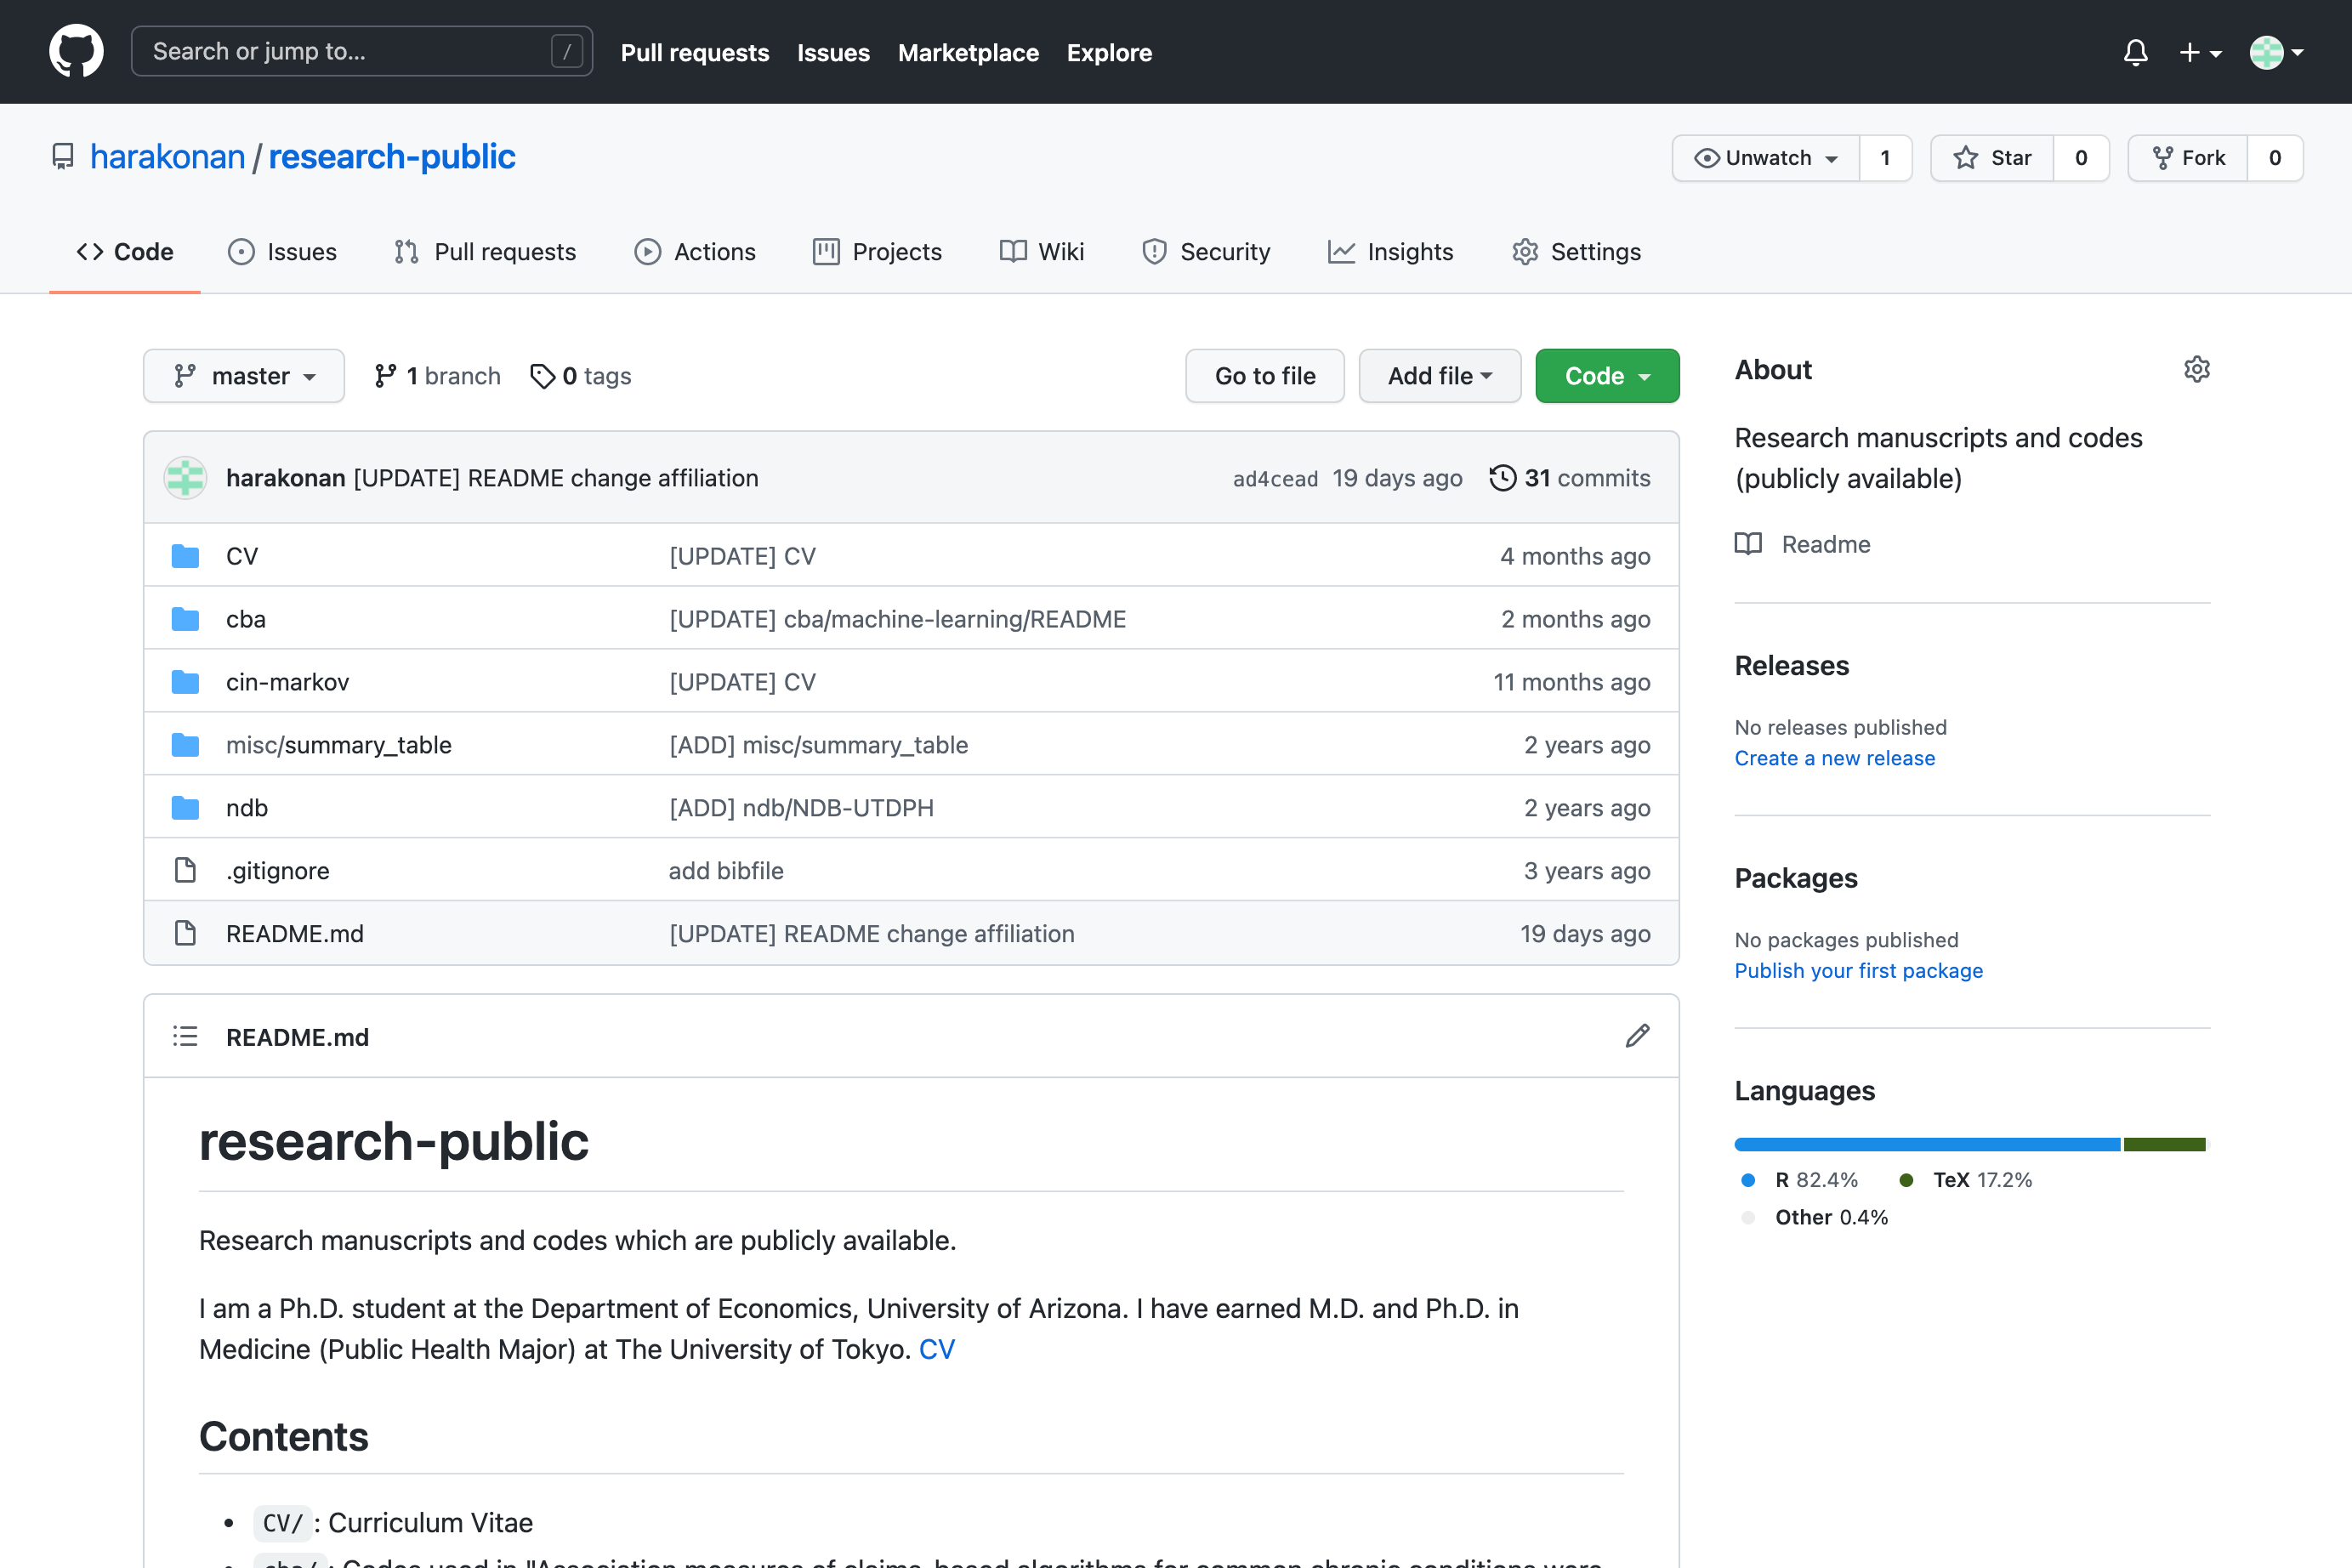
\includegraphics[width=0.9\textwidth]{fig/github_public.png}
	\end{figure}

	\end{frame}

	\begin{frame}
	\frametitle{GitHub Can Help You: README File}
	\begin{figure}
	\only<1>{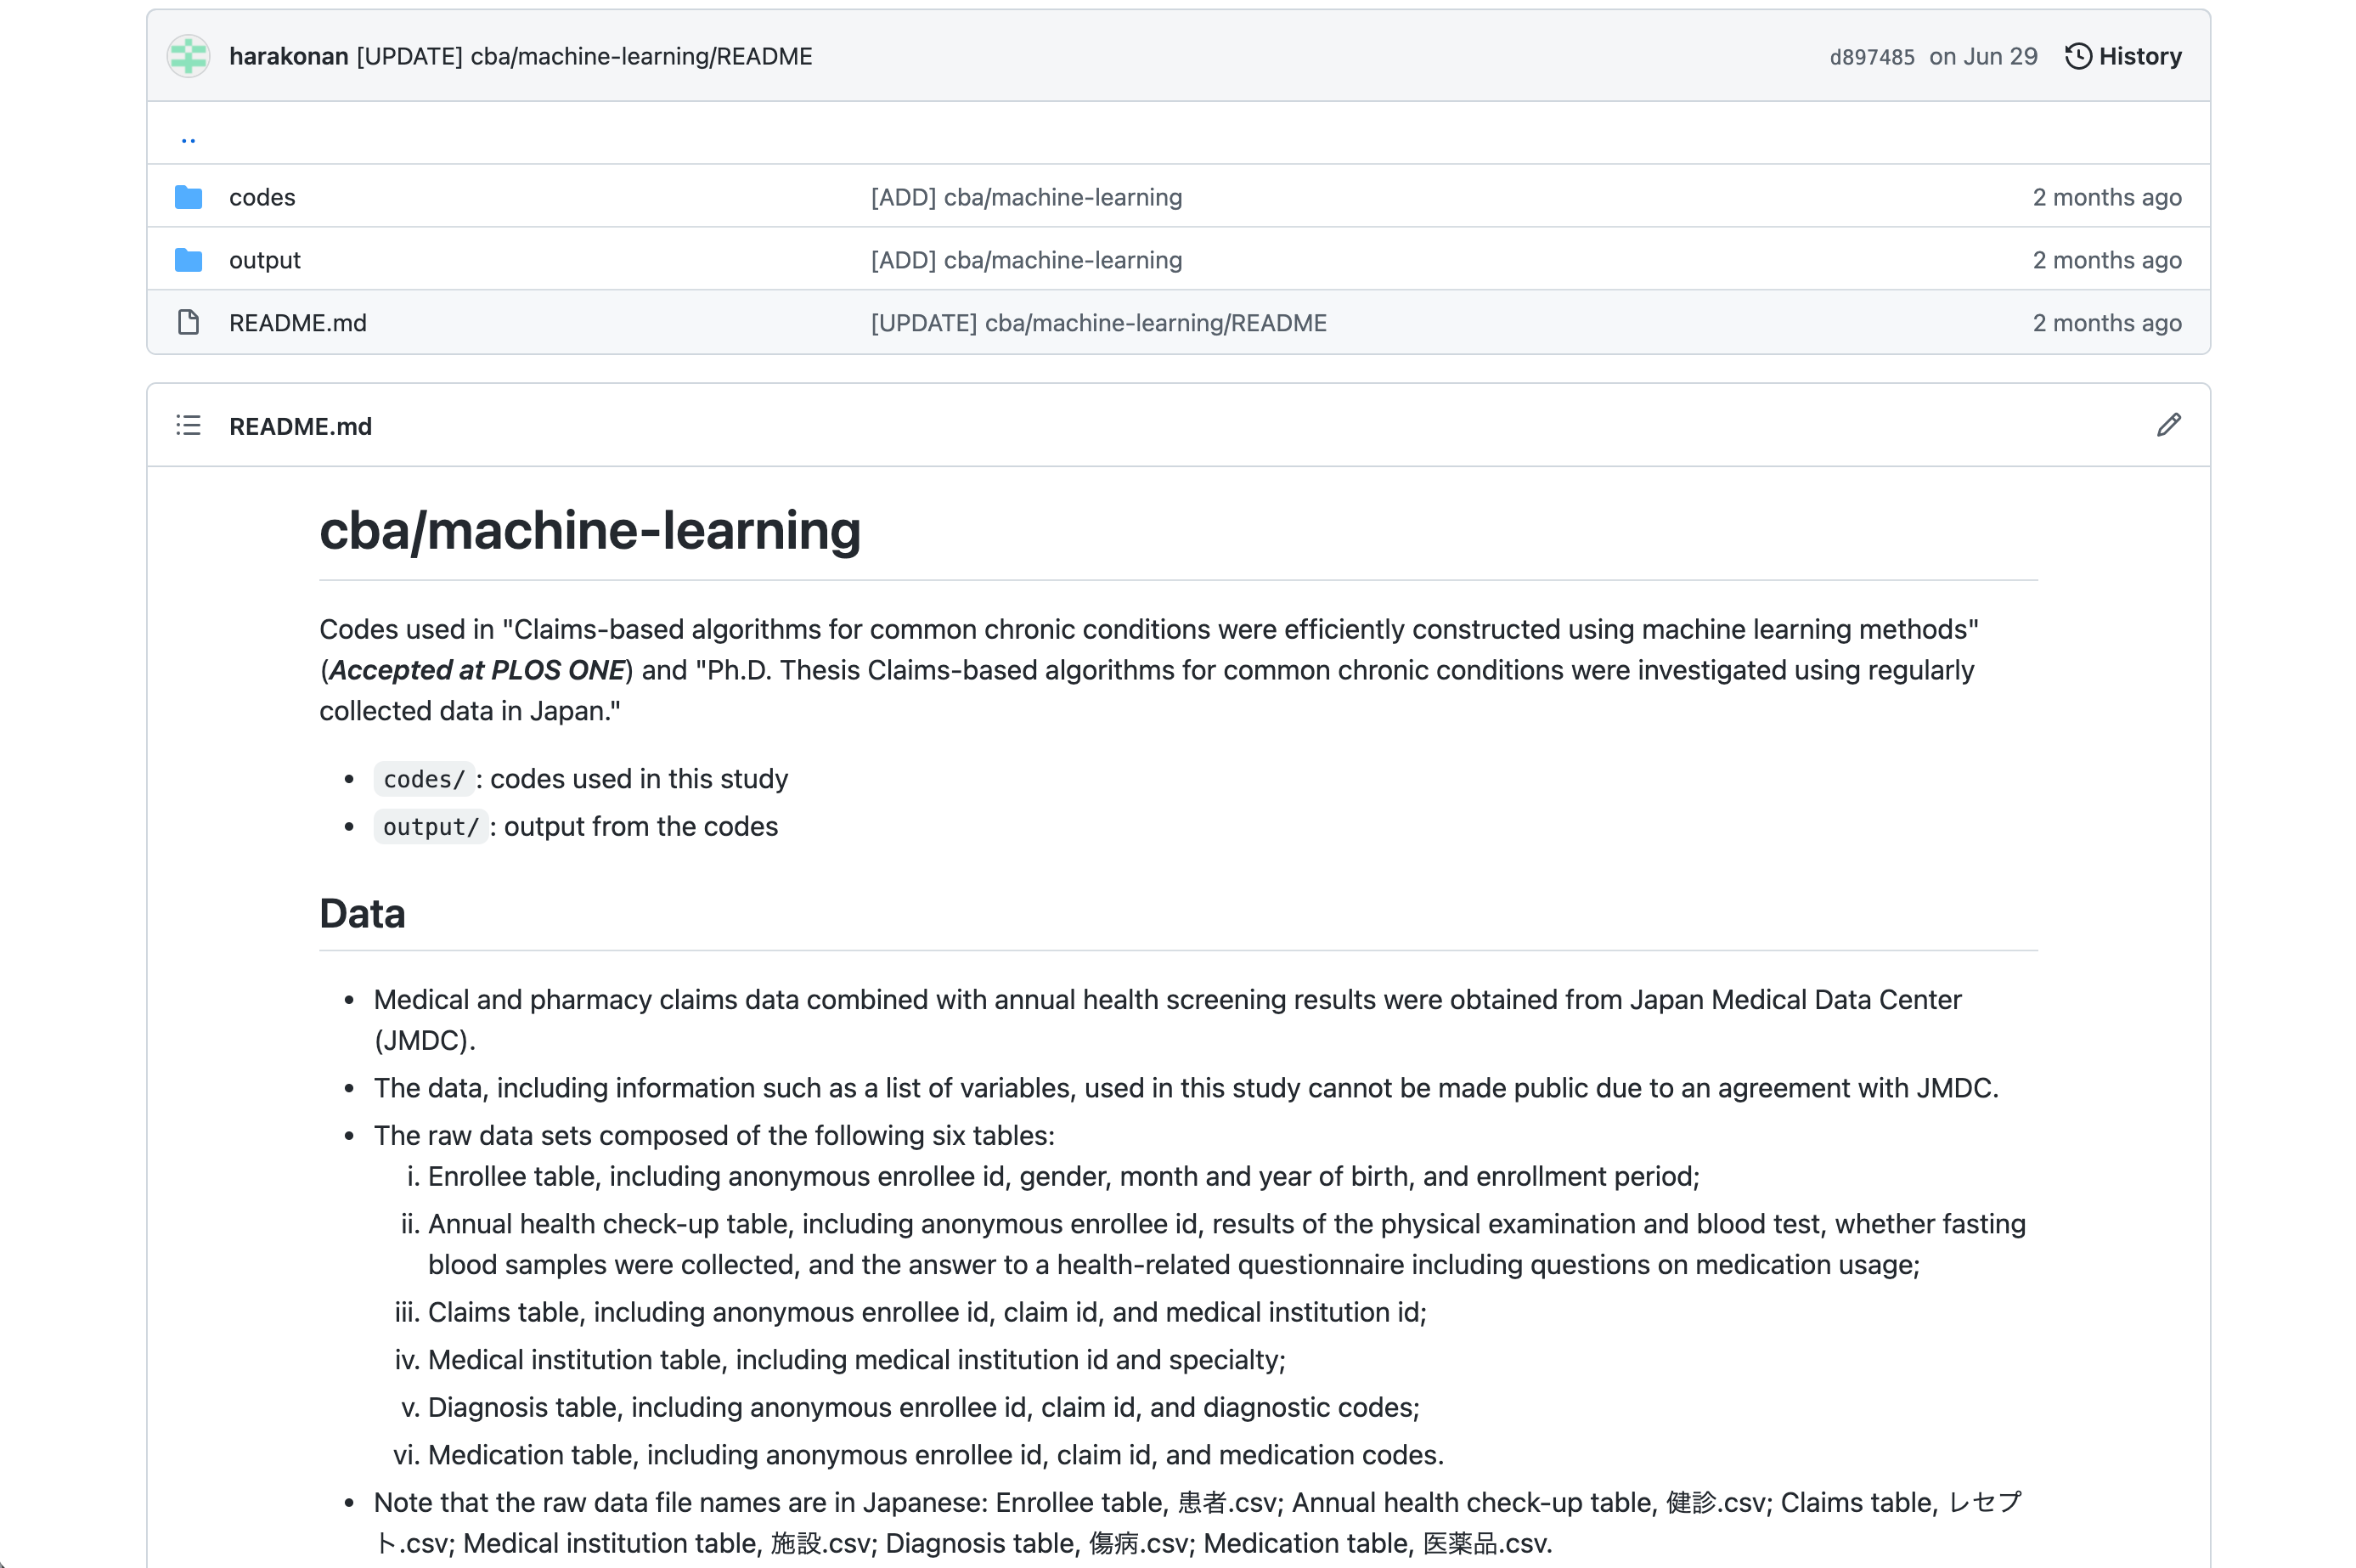
\includegraphics[width=0.9\textwidth]{fig/github_readme1.png}}
	\only<2>{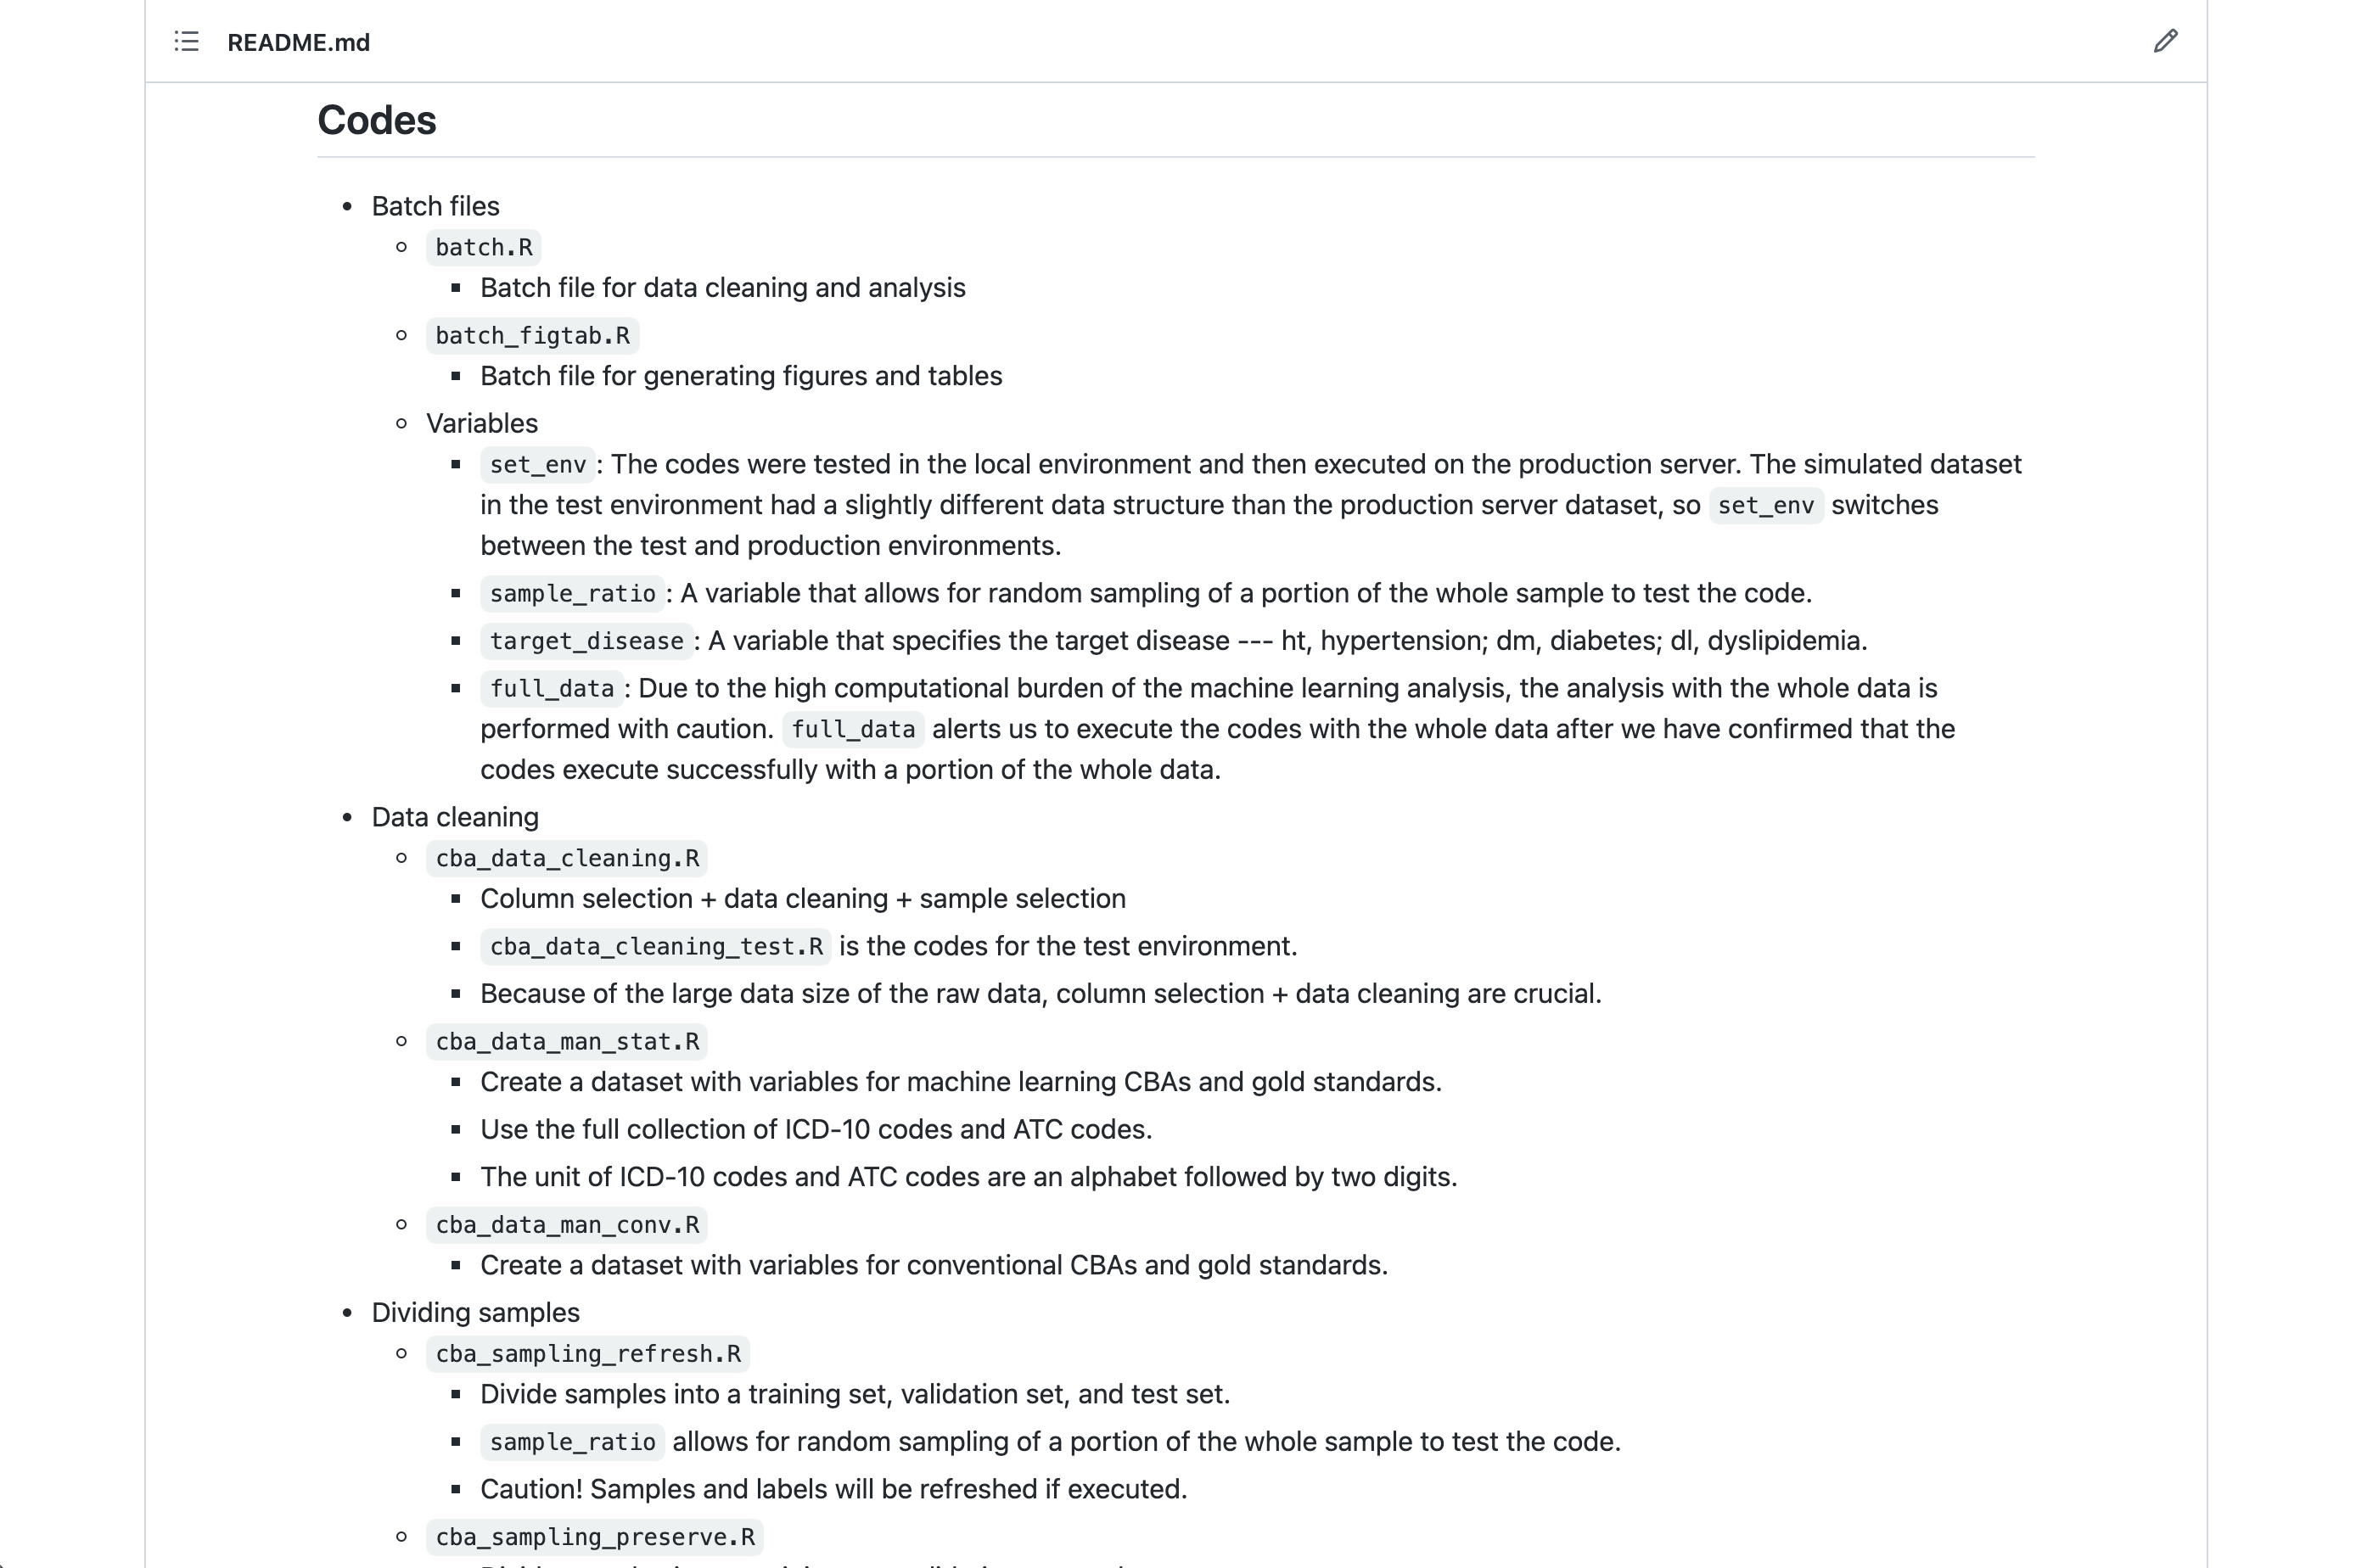
\includegraphics[width=0.9\textwidth]{fig/github_readme2.png}}
	\only<3>{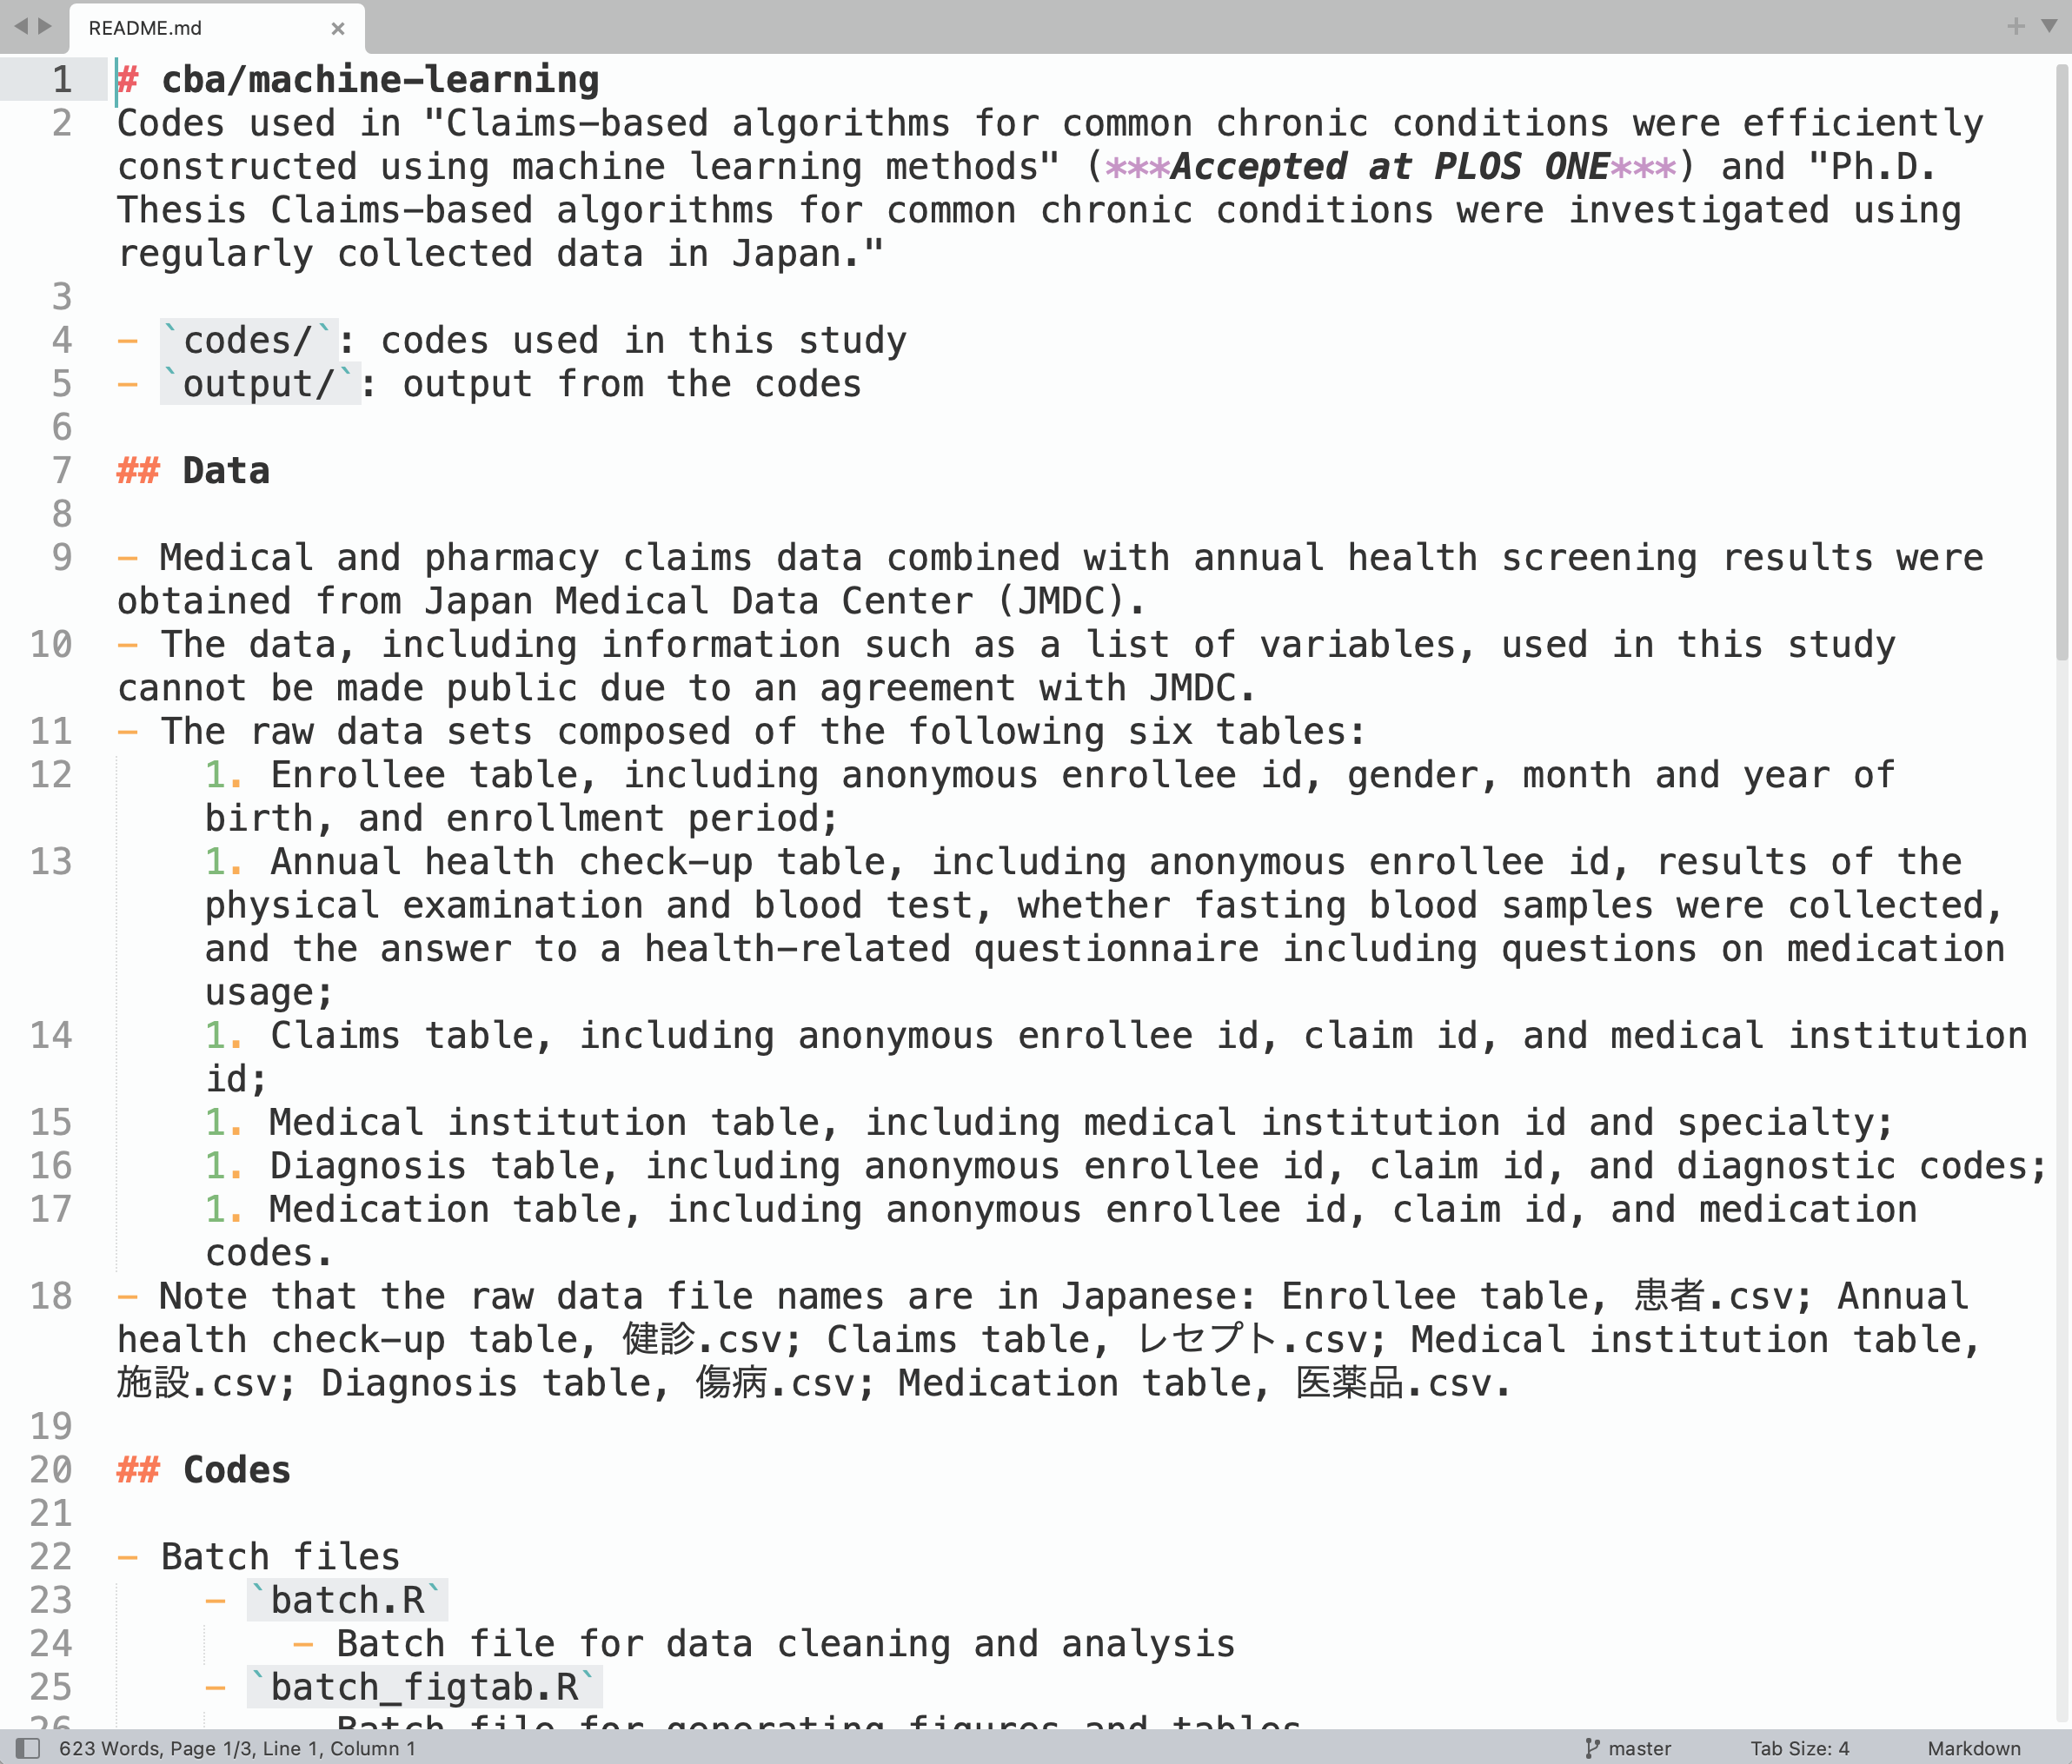
\includegraphics[width=0.9\textwidth]{fig/github_readme3.png}}
	\end{figure}

	\end{frame}

	\begin{frame}
	\frametitle{GitHub Can Help You: Modification History}
	\begin{figure}
	\only<1>{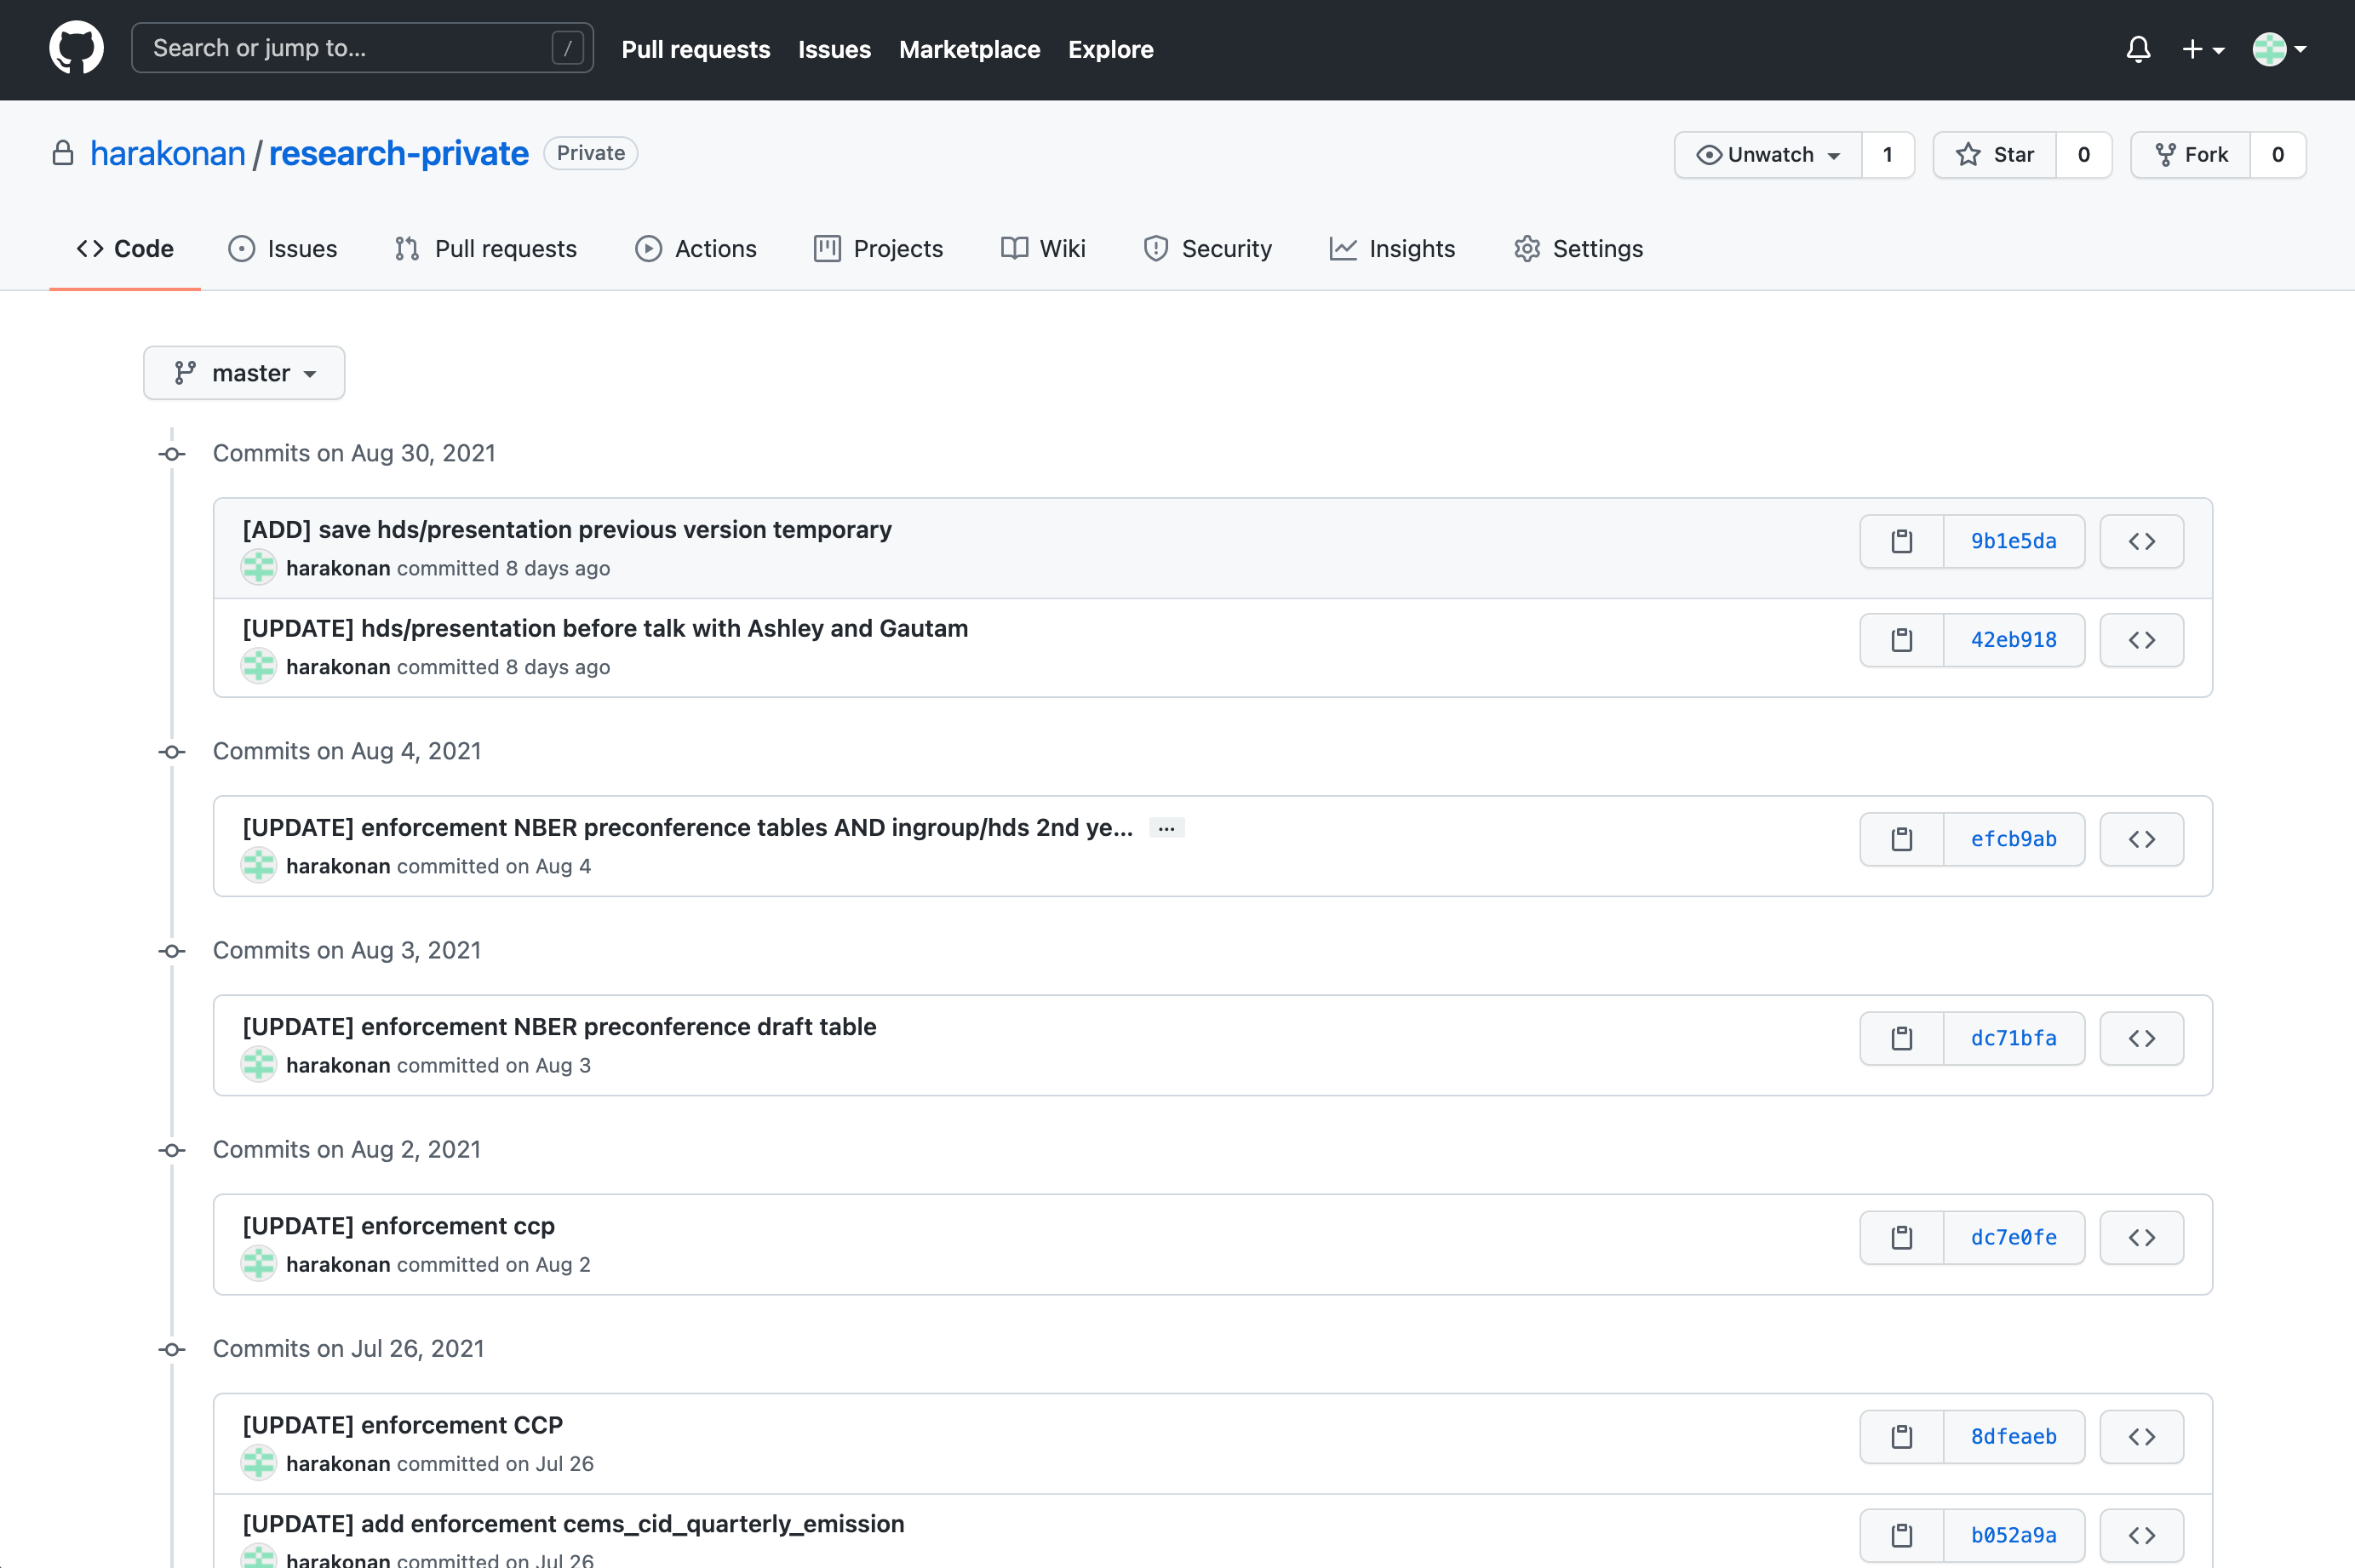
\includegraphics[width=0.9\textwidth]{fig/github_modification_history1.png}}
	\only<2>{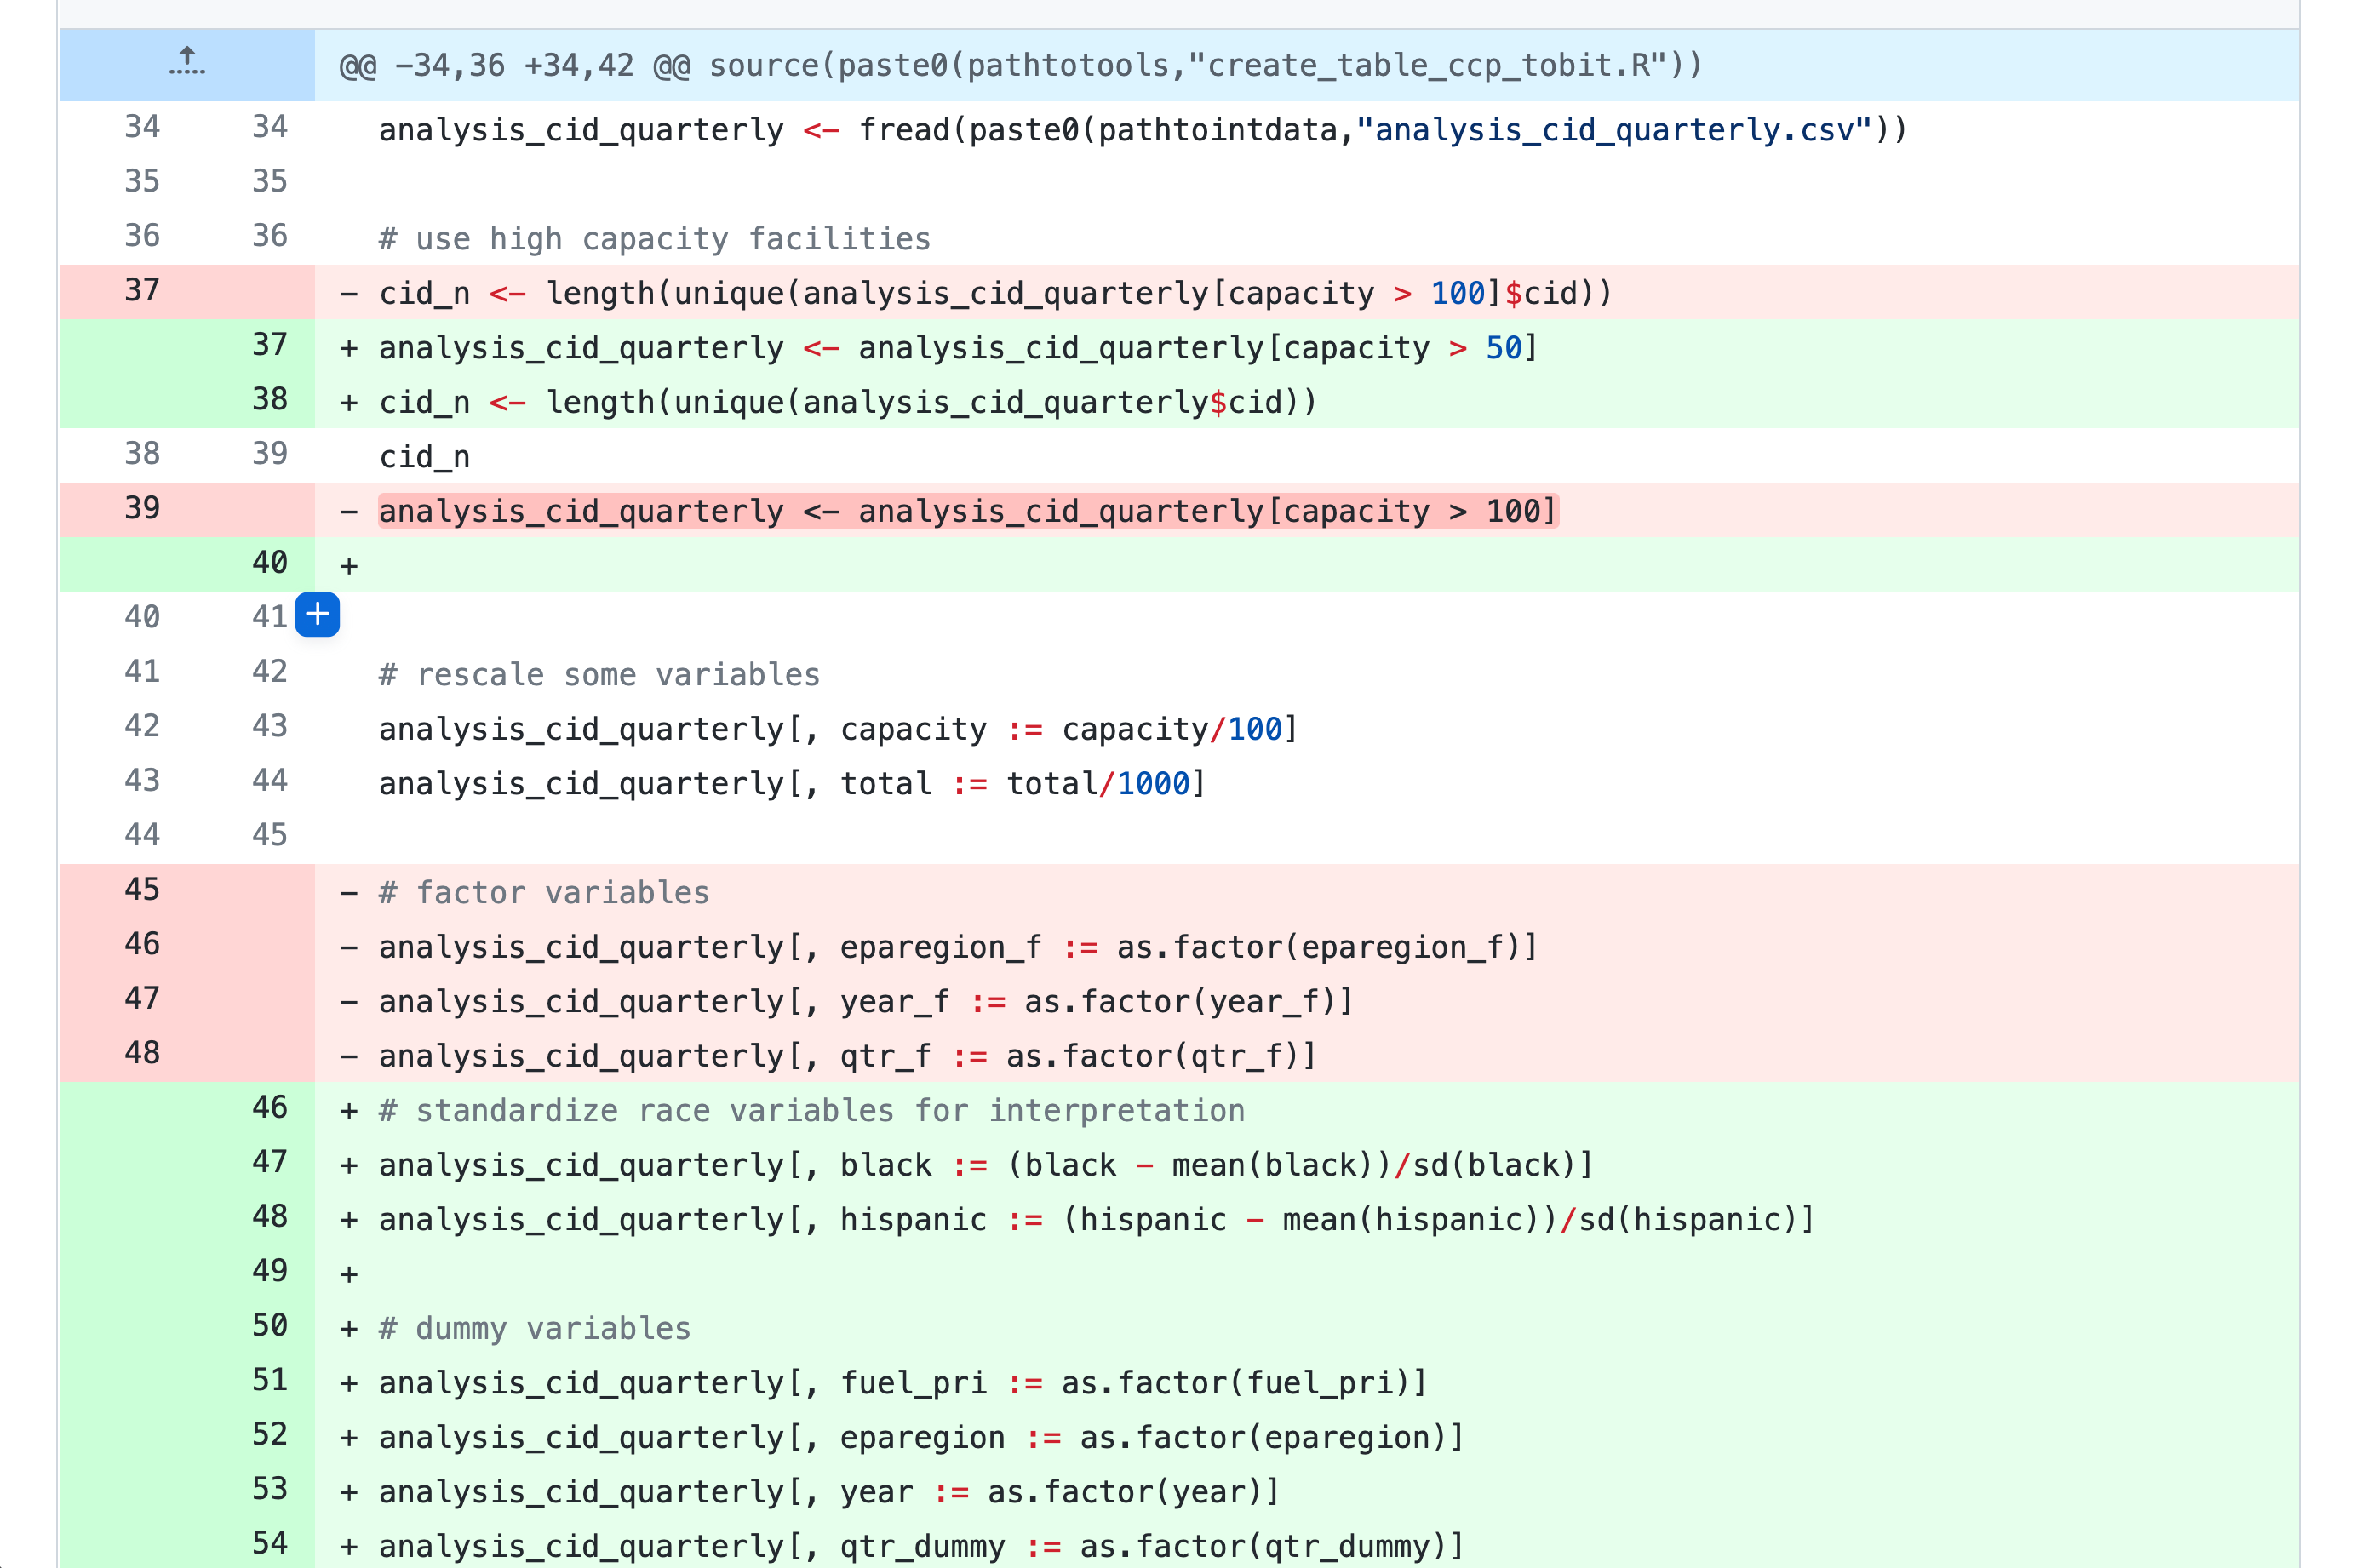
\includegraphics[width=0.9\textwidth]{fig/github_modification_history2.png}}
	\end{figure}

	\end{frame}

	\begin{frame}
	\frametitle{Reproducible Research Using R: R Markdown}
	\begin{figure}
	\only<1>{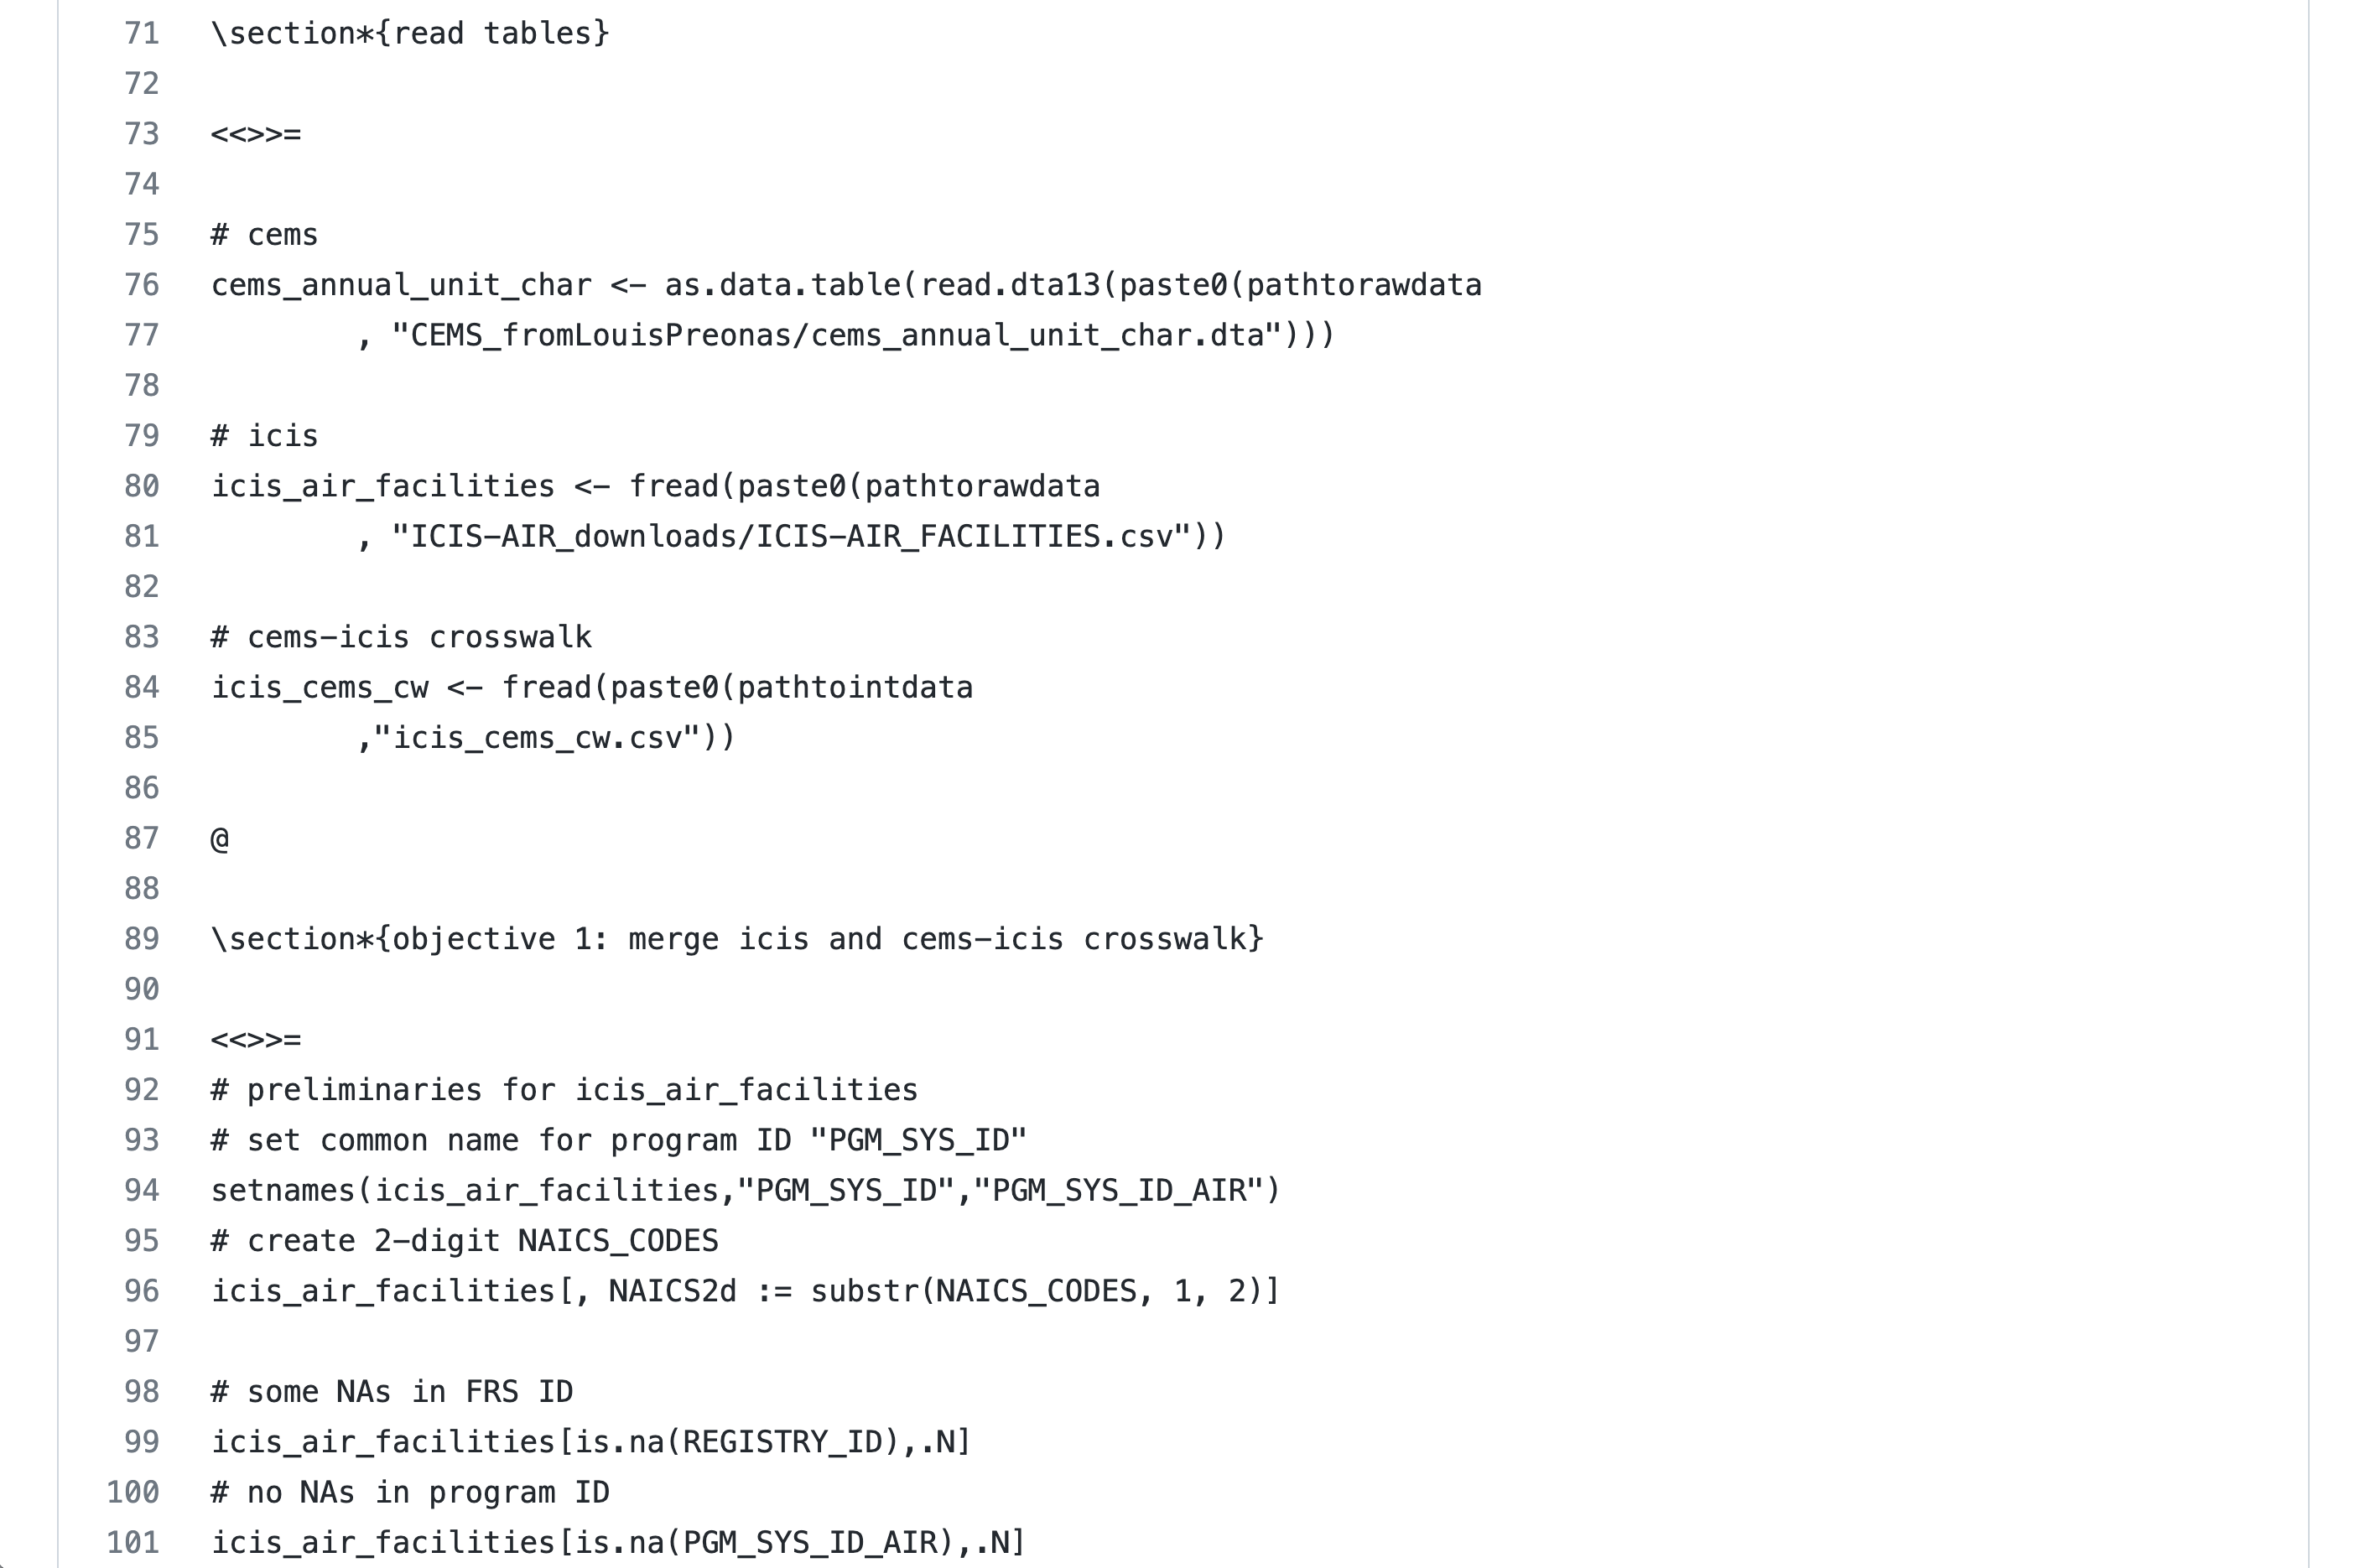
\includegraphics[width=0.9\textwidth]{fig/reproducible1.png}}
	\only<2>{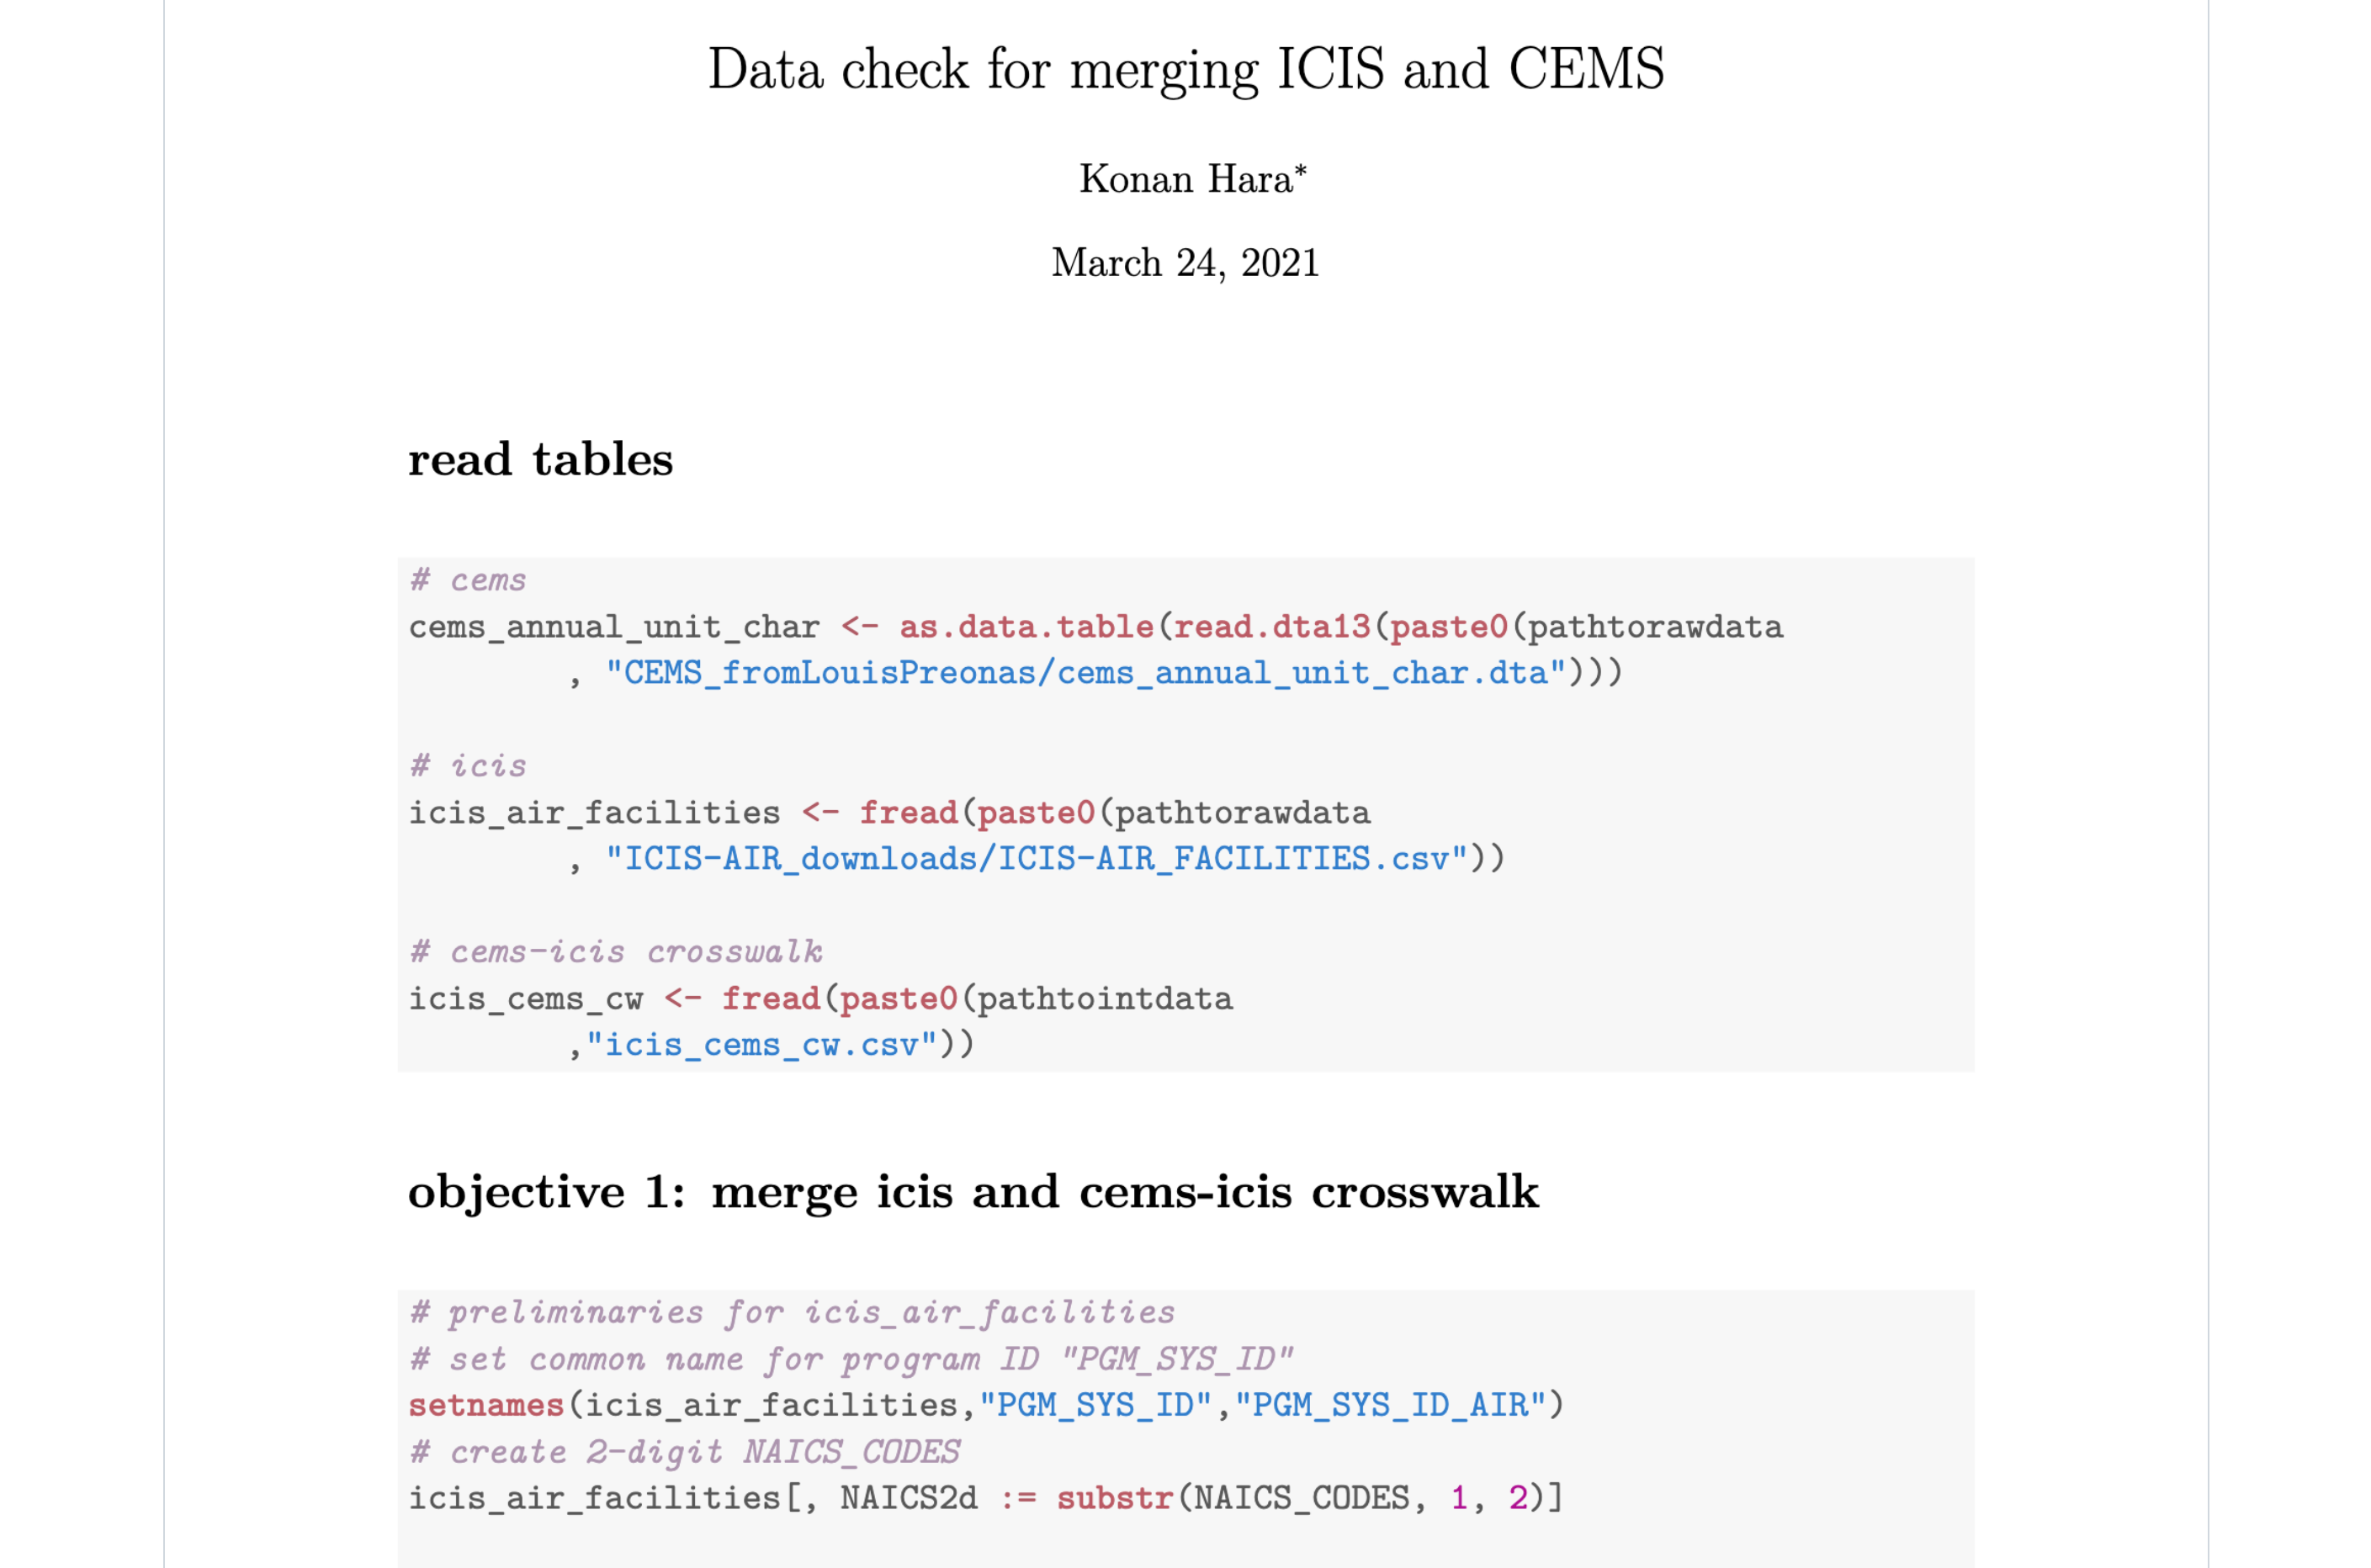
\includegraphics[width=0.9\textwidth]{fig/reproducible2.png}}
	\only<3>{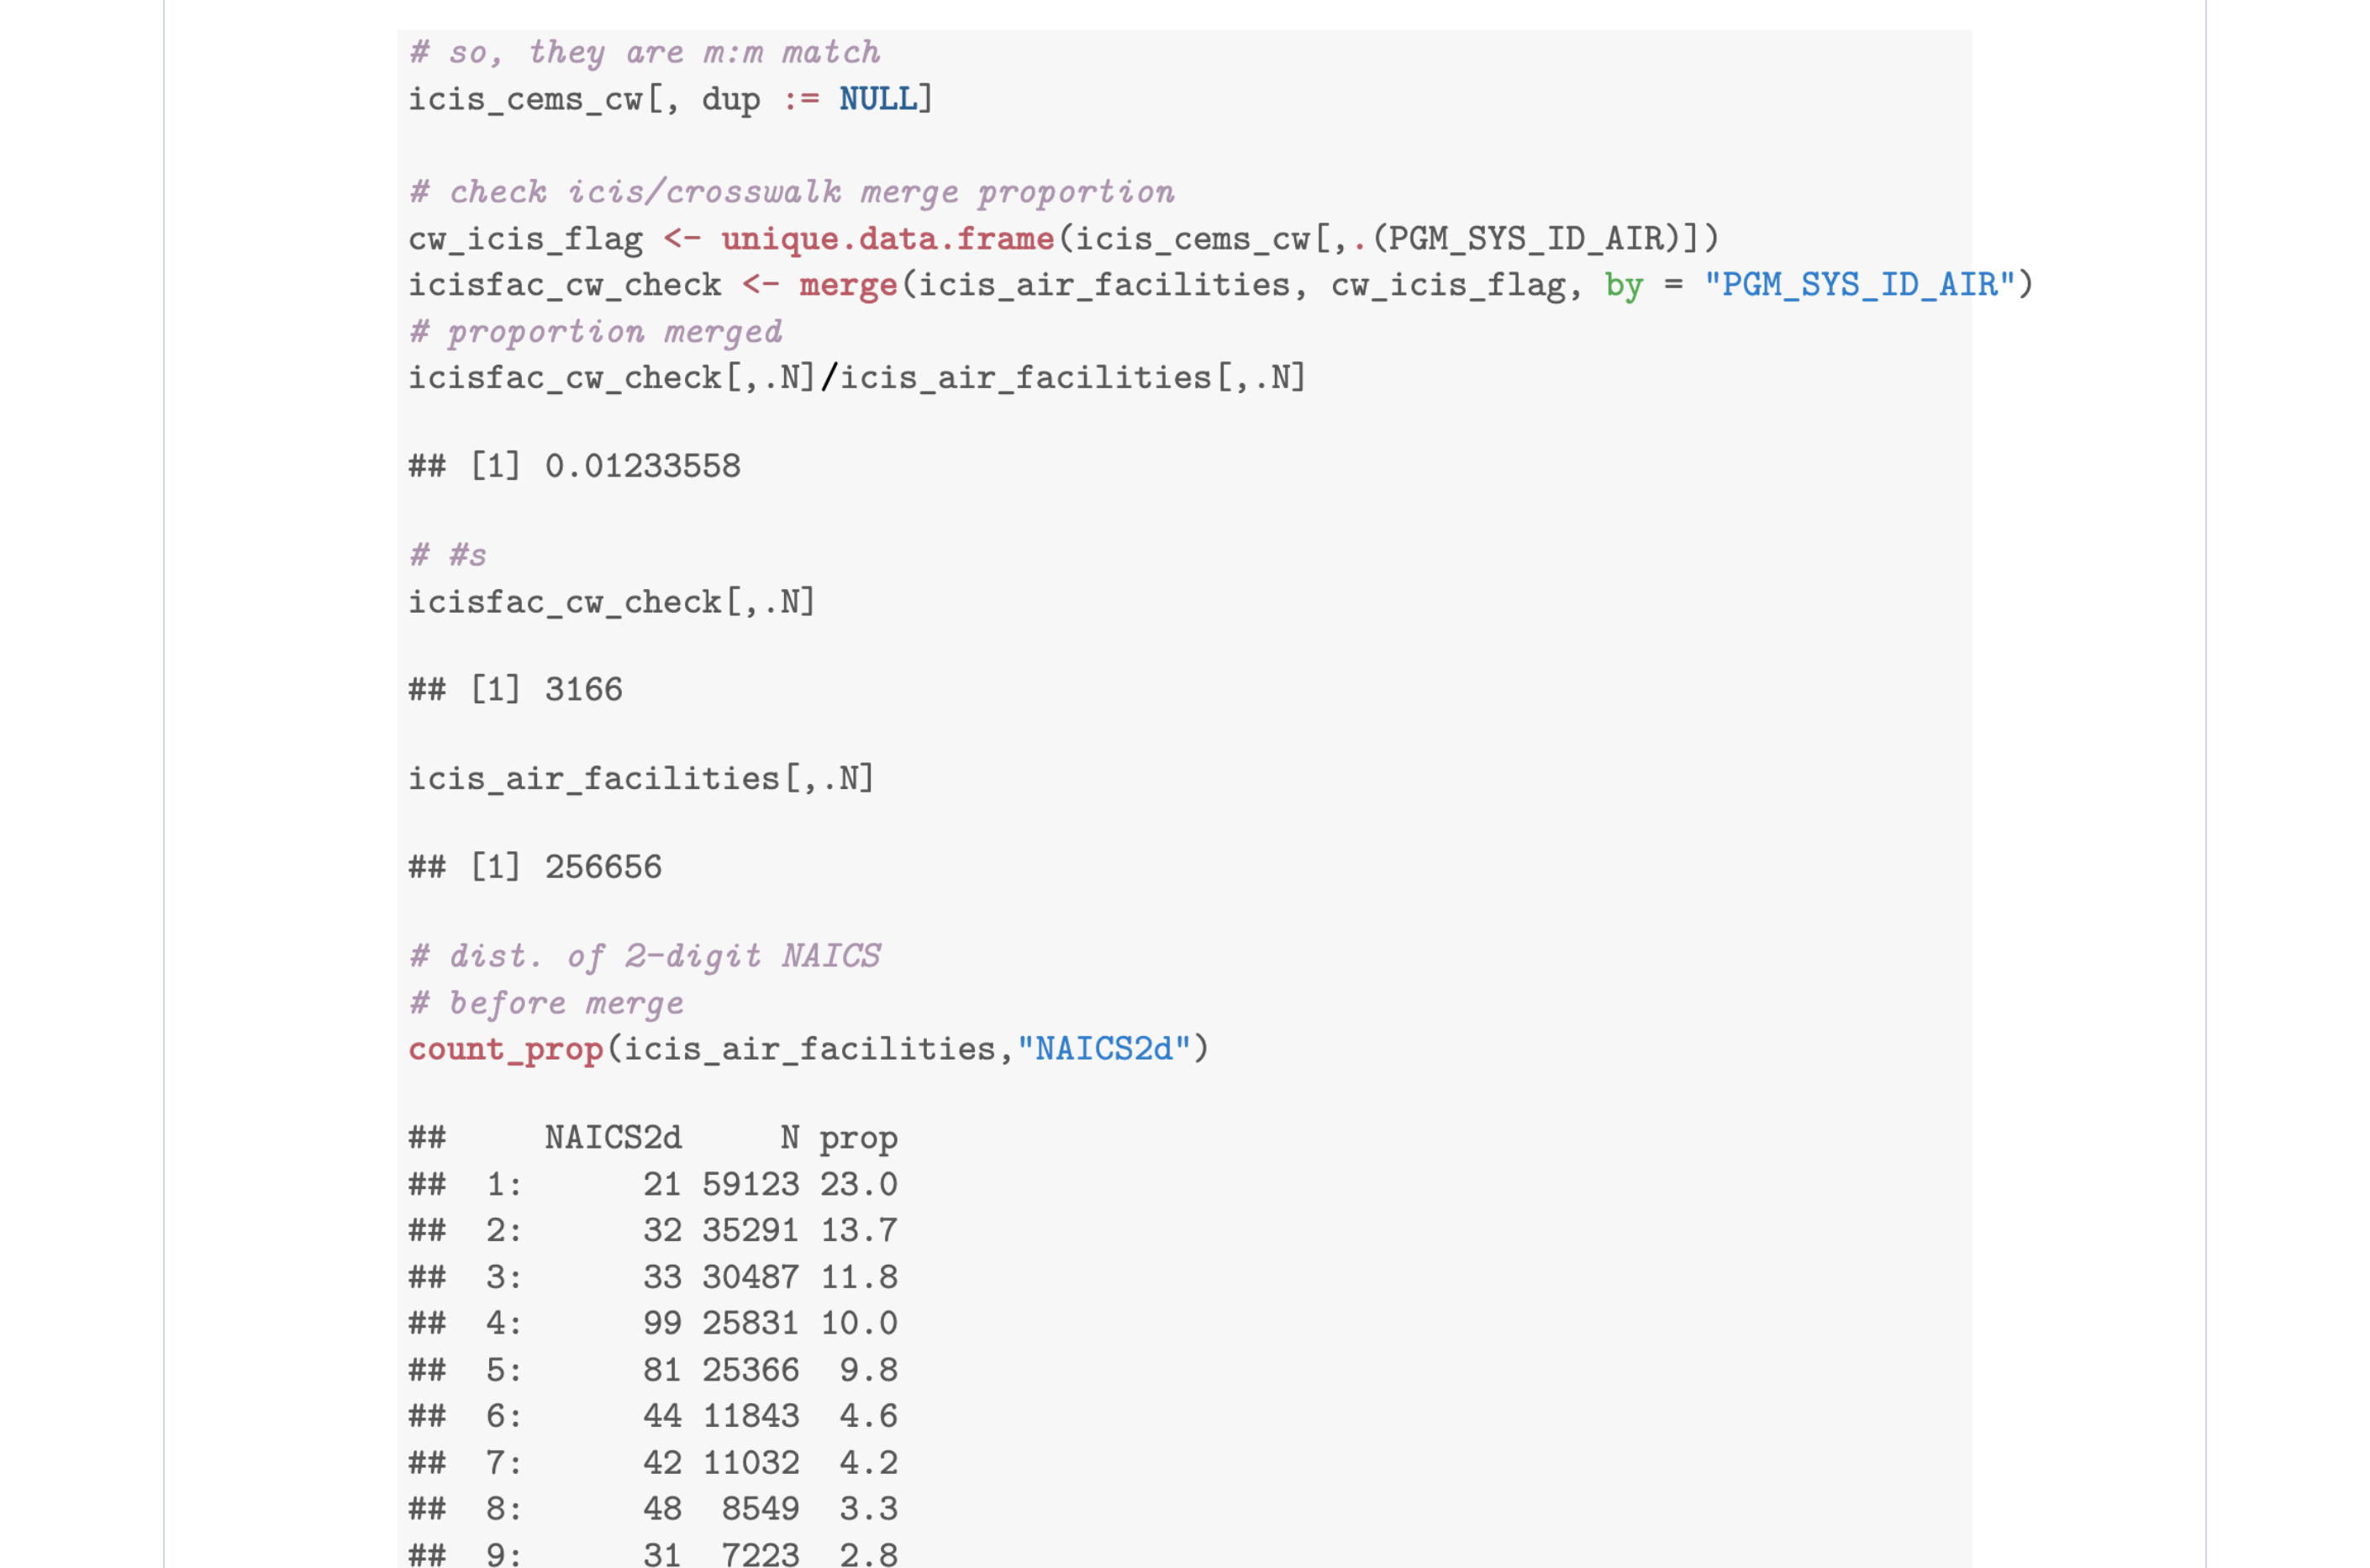
\includegraphics[width=0.9\textwidth]{fig/reproducible3.png}}
	\only<4>{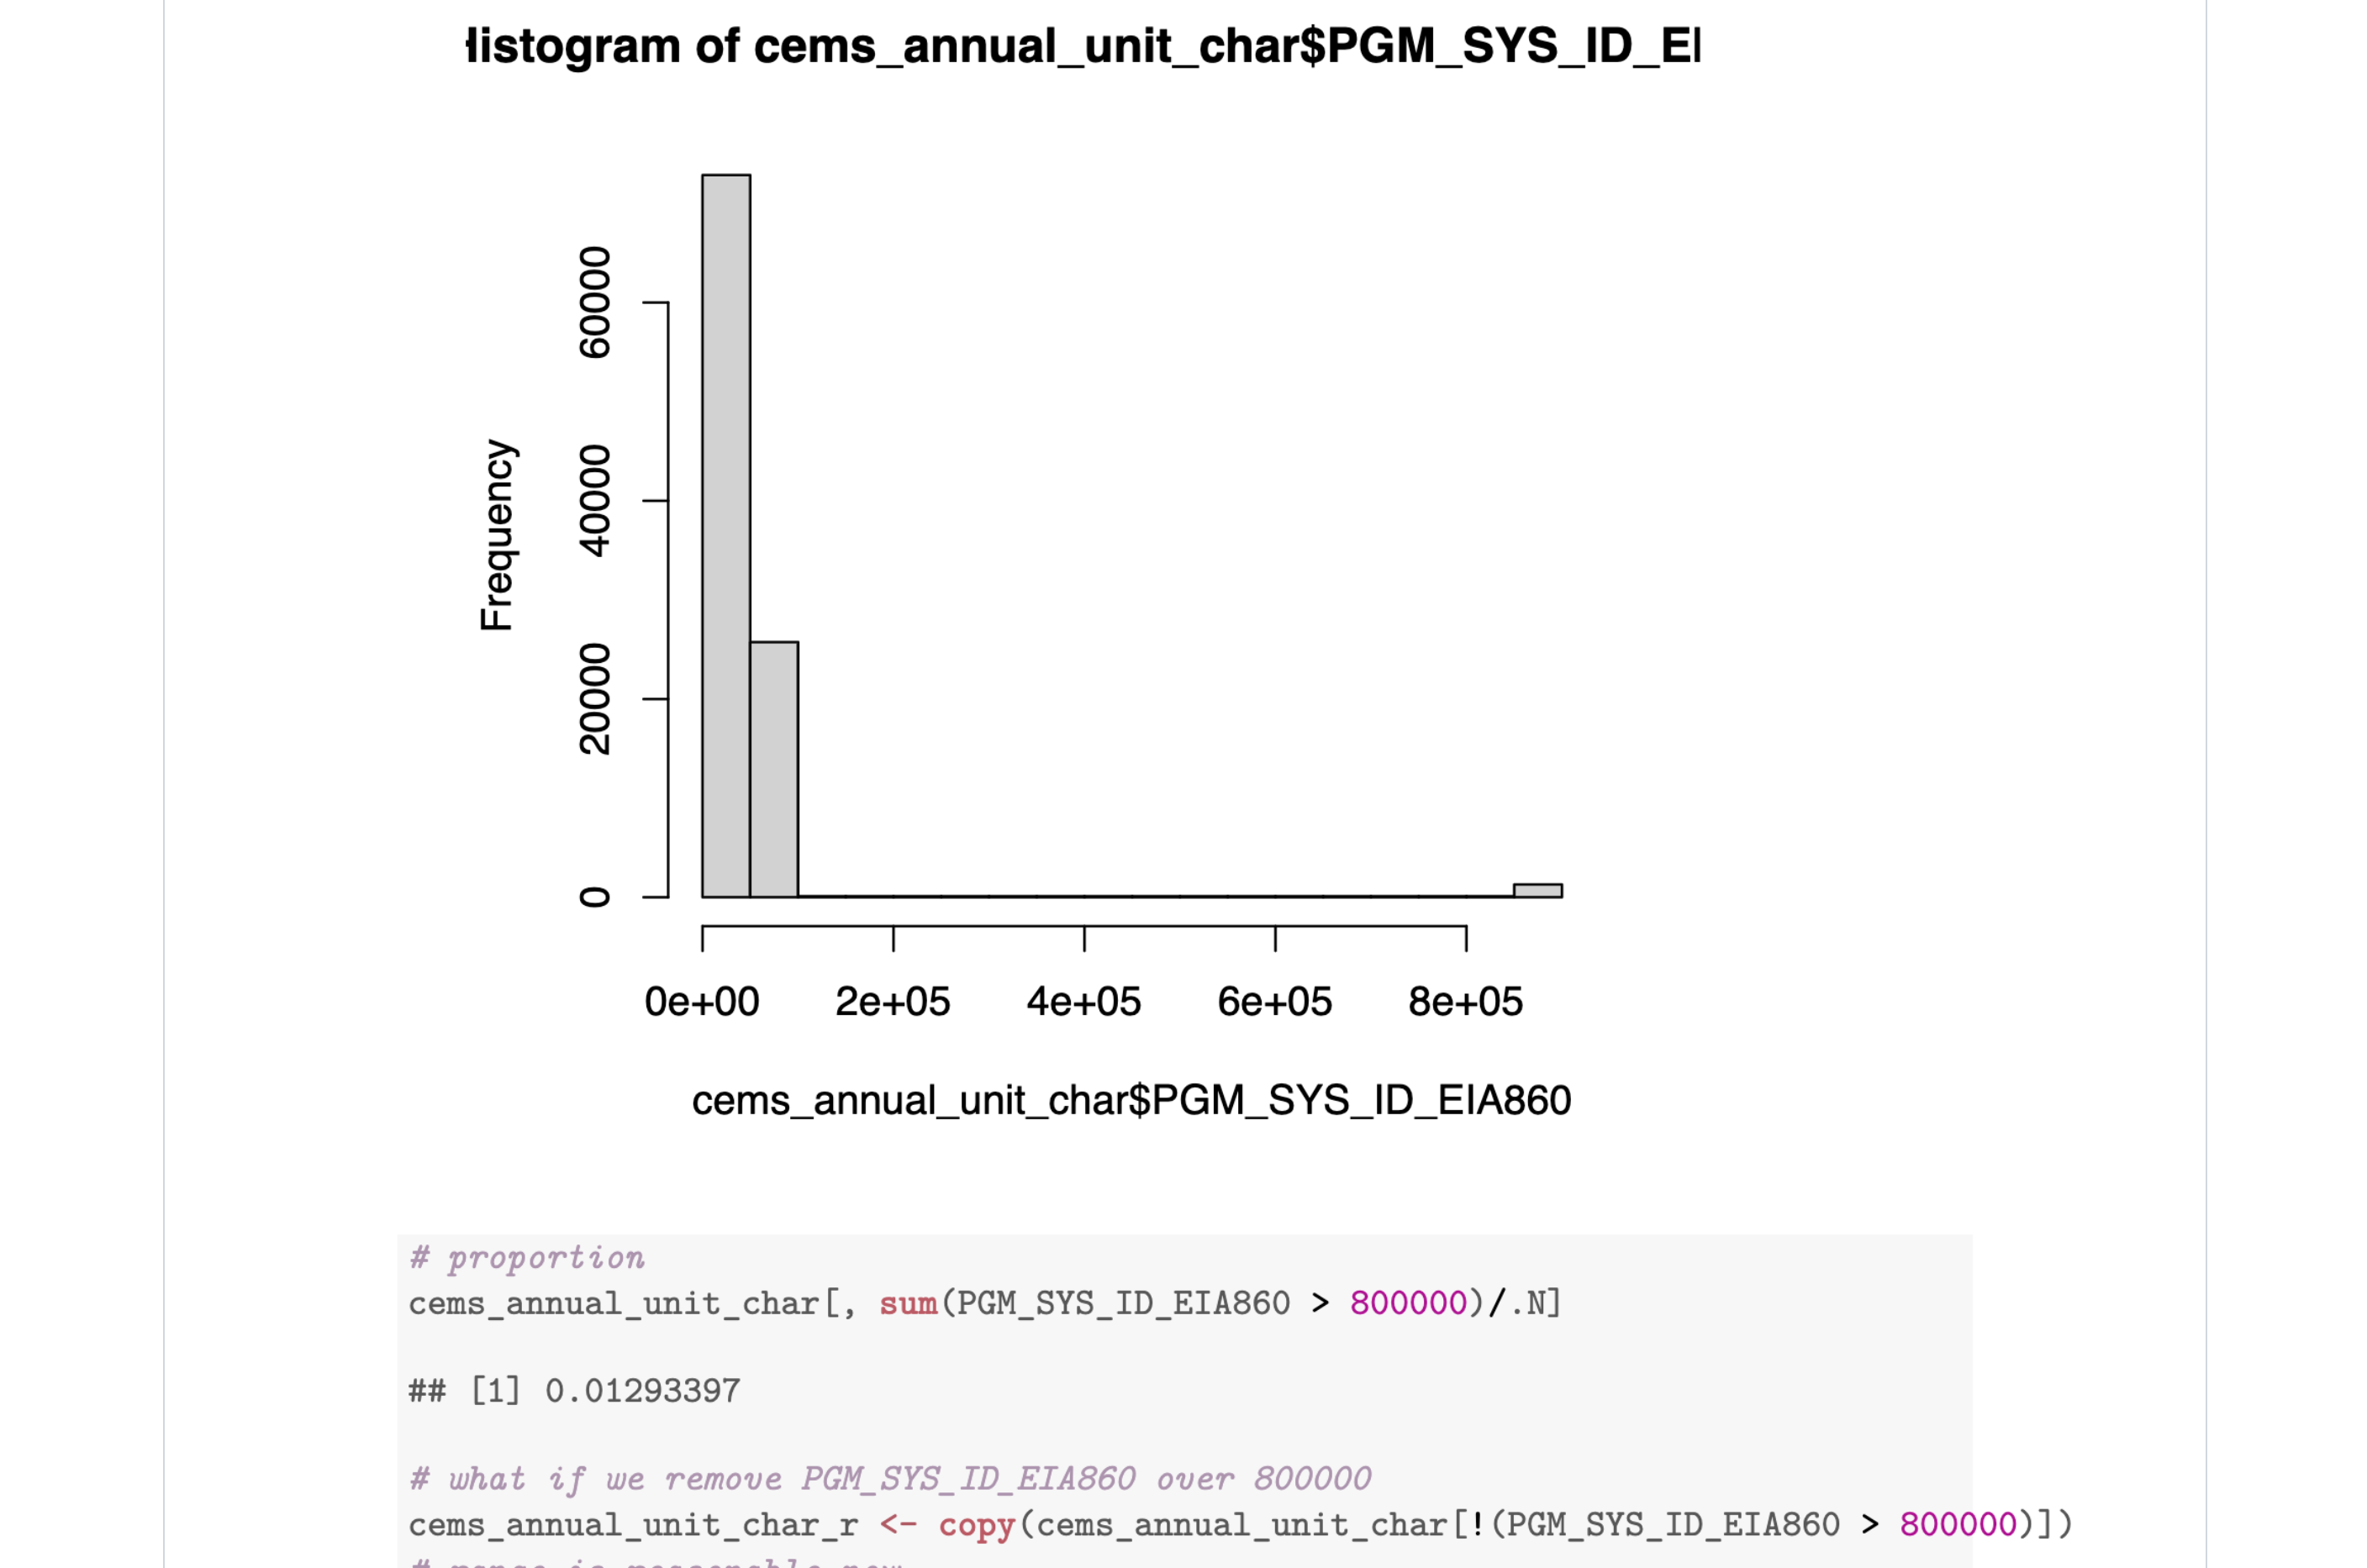
\includegraphics[width=0.9\textwidth]{fig/reproducible4.png}}
	\end{figure}

	\end{frame}

	\begin{frame}
	\frametitle{Programming Habits: Demonstration}
	\begin{enumerate}
	\item Change codes in a R markdown file
	\item Execute them to check whether they work
	\item Compile the R markdown file
	\item Track changes using GitHub
	\end{enumerate}

	\end{frame}

	\begin{frame}
	\frametitle{Example R Codes}
	Topics\_on\_R\_example\_codes.pdf demonstrates some R codes examples:
	\begin{enumerate}
	\item Getting Help
	\item R Objects
	\item Loops
	\item Regressions
	\item Plots
	\item User-defined Functions and Optimization
	\end{enumerate}

	\end{frame}


	\begin{frame}
	\frametitle{Import a Dataset}
	\begin{itemize}
	\item Csv file
	\begin{itemize}
	\item data.frame way: read.csv()
	\item data.table way: fread()
	\item tibble way: read\_csv()
	\end{itemize}
	\item Other file formats (using haven package)
	\begin{itemize}
	\item SAS: read\_sas()
	\item SPSS: read\_sav()
	\item Stata: read\_dta()
	\end{itemize}

	\end{itemize}

	\end{frame}

	\begin{frame}
	\frametitle{Lots of Others Things With R}
	\begin{itemize}
	\item Potential topics
	\begin{itemize}
	\item Web scraping
	\item Natural language processing
	\item Image recognition
	\end{itemize}
	\item Learning plantforms:
	\begin{itemize}
	\item \href{https://www.coursera.org/}{\underline{Coursera}}
	\item \href{https://www.datacamp.com/onboarding}{\underline{Datacamp}}
	\end{itemize}

	\end{itemize}

	\end{frame}



















\end{document}
